\documentclass[final,journal,letterpaper]{IEEEtran}

\usepackage{cite}
\usepackage{amsmath}
\usepackage{amsfonts}
\usepackage{amssymb}
\usepackage{graphicx}
\usepackage{url}
\usepackage{balance}
\usepackage{float}
\usepackage{threeparttable}

\usepackage[T1]{fontenc}
\usepackage[latin9]{inputenc}
\usepackage{textcomp}
\usepackage{mathrsfs}
\usepackage{amsthm}

\usepackage{mathptmx}
\usepackage[scaled=.90]{helvet}
\usepackage{courier}

\usepackage{color}

\usepackage{listings}
\usepackage{listings}

\lstset{
   language=C,
   basicstyle=\small,
   keywordstyle=\bfseries,
   identifierstyle=\ttfamily,
   stringstyle=\ttfamily,
   numbers=left,
   numberstyle=\tiny,
   stepnumber=1,
   numbersep=-5pt,
   showstringspaces=false
%   frame=single %trbl%
}

\usepackage[normalem]{ulem}

%------------------------------------------------------------------------------

\newcommand{\etal}{\emph{et al.}}
\newcommand{\eg}{\emph{e.g.}}
\newcommand{\ie}{\emph{i.e.}}
\newcommand{\etc}{\emph{etc.}}

%\newcommand{\comment}[1]{\textcolor{red}{AA: \bf #1}}
\newcommand\comment[1]{} % When you enable this lines, all the notes will disappear


%\renewcommand{\baselinestretch}{0.98}\normalsize
%------------------------------------------------------------------------------
\makeatletter
%%%%%%%%%%%%%%%%%%%%%%%%%%%%%% Textclass specific LaTeX commands.
\theoremstyle{plain}
\newtheorem{thm}{\protect\theoremname}
\theoremstyle{definition}
\newtheorem{defn}{\protect\definitionname}
\theoremstyle{remark}
\newtheorem{rem}{\protect\remarkname}

%\newtheorem{defn}[thm]{\protect\definitionname}
%\theoremstyle{remark}
%\newtheorem{rem}[thm]{\protect\remarkname}
%\makeatother

%\usepackage{babel}
\providecommand{\definitionname}{Definition}
\providecommand{\remarkname}{Remark}
\providecommand{\theoremname}{Theorem}

\begin{document}

\author{Vincenzo~Catania, Andrea Araldo~and~Davide~Patti% 
\thanks{The authors are with the Dipartimento di Ingegneria
Elettrica, Elettronica ed Informatica, Universit\`a di Catania, Italy
(email: \{vincenzo.catania,aaraldo,davide.patti\}@dieei.unict.it).}}

\title{Parameter Space Representation of Pareto Front to
Explore Hardware-Software Dependencies}
%ATTENZIONE: in questo testo io mi sono riferito a ``Pareto set''
%come un sottoinsieme dello spazio degli obiettivi (vedi, ad es., descrizione
%dell'algoritmo). E' pi� corretto forse, invece, intendere il Pareto
%set come un sottoinsieme dello spazio delle configurazioni.

\maketitle
\begin{abstract}
Embedded Systems Design often requires conflicting objectives to be
optimized with an appropriate choice of hardware/software parameters .
Interdependencies among these parameters can make this task even more
difficult, since an a-priori knowledge of them would  be required to
develop an analytical model of the system. In this work we present PS,
a multiobjective exploration strategy that introduces the notion of
Parameters Space Representation. After a detailed formal description
of the algorithm and its concepts, we show a hardware/software
exploration case study. Qualitative and quantitative comparisons of PS
against a well-know multiobjective genetic approach demonstrate that,
while not outperforming it in terms of dominance, the proposed
approach can trade the uniformity and granularity qualities of the
solutions found for obtaining larger Pareto sets, thus representing a
further choice for designer when objective constrains allow it.
\end{abstract}

%------------------------------------------------------------------------------
%\IEEEkeywords{...}

\begin{IEEEkeywords}
DSE, MultiObjective Optimization, Genetic Algorithms
\end{IEEEkeywords}
%------------------------------------------------------------------------------

\section{Introduction and Motivation}
\comment{Si capisce che noi provide an algorithm?}

\comment{Mettere our contribution?}

\comment{Usare triangleq quando definiamo noi le cose, per distinguerlo dall'= di calcolo}

The design of an embedded system requires different conflicting
objectives (energy consumption, performance, area) to be fulfilled.
Several factors are involved in this goal and real cases show how
often no analytical results are known to predict the relation between
system configurations and objectives. In such cases a high level
system simulation is often the only way to have a picture of how system
parameters impact on the objectives.  A key problem is that the size
of the design space to be simulated grows with the product of
cardinalities of each parameter, easily resulting in an intractable number
of simulations. In these cases a ``Design Space
Exploration'' strategy is required, i.e. a methodology to evaluate
only a small subset of all possible configurations while maintaining a
good level of efficiency and accuracy~\cite{surviving_soc}.

The final result of a design space exploration is a subset of the
configurations called Pareto Set (\cite{pareto}) (See also Definition
\ref{pers02.def:Pareto-set}). It represents the trade-offs between
objectives, so that for each configuration of the Pareto Set there is no
other configuration performing better for all the objectives
considered. Once these few promising configurations have been obtained, a
subsequent step of the design flow can eventually afford a more
accurate low level simulation.

In this work we present a multiobjective design exploration strategy
that introduces the concept of Parameter Space Representation of
Pareto Set (PS).\comment{Provo a fare il reviewer stronzo. Allora, quando parliamo di parameter space, non si capisce bene di cosa parliamo. Alla fin fine penso (ma gia' se nemmeno io che ci ho messo mano ne sono sicuro, figuriamoci il reviewer) stiamo parlando del configuration space, che definiamo precisamente nella \secR{pareto}. In altre parole parameter space == configuration space. Quindi, visto che il Pareto set e' contenuto nel configuration space, il Pateto-set e' gia', lui stesso, una Parameter Space Representation of Pareto-set. E' come dire ``io sono la rappresentazione di me stesso'', che filosoficamente e' affascinante ma matematicamente non lo e' altrettanto!} The main idea is focusing on the ``innovation''
introduced in the Pareto sets and then accordingly distributing the
exploration effort in regions created in the multidimensional space of
system parameters. The aim of the PS approach is to propose a new
perspective on the configuration space, where parameter
interdependencies play the fundamental role of making some regions
more capable of generating hardly predictable solutions: catching this
sort of ``chaoticity'' in the parameter space is the main idea behind
the strategy that is being introduced in this work.

\section{Related work and Contribution}
\label{sec:Related-work}
Many different design space exploration algorithms have been proposed
in literature.  The motivations of an exploration
algorithm are rather heuristic, have some form of arbitrariness and,
to a large extend, intuition lies behind them.

Some exploration strategies assume some kind of knowledge about the
system parameters, their meaning and their impact on design
objectives.  The \emph{Dependency analysis}, proposed in
\cite{givargis_tvlsi02}, is meant to take advantage of the parameter
dependencies. Starting from them, he can construct a ``dependency graph''
and recognize clusters, i.e. subsets of strongly dependency-connected
parameters. Each cluster is exhaustively evaluated and its ``local''
Pareto set is found. Then, all local Pareto sets are merged. In this
way, a series of local exhaustive evaluations are performed instead of
an exhaustive evaluation of all the possible configurations. Some
problems arise: i) In real scenarios, it may be difficult to recognize
really independent clusters of parameters, because there may be
interdependencies among a large number of parameters. This may lead to
the need of an evaluation of almost all the possible configurations.
ii) A designer may not have a precise and complete a-priori picture of
the dependencies among parameters; for this reason the need of
``automated approaches for computing interdependencies'' is declared
in the same paper.  These drawbacks are not present in our algorithm,
since, although it leverages dependencies as in
\cite{givargis_tvlsi02}, it is able to detect them automatically, with
no a-priori knowledge required. Moreover, our algorithm is able to
capture also ``local dependencies", i.e. dependencies that emerge only
among certain ranges of parameters and may not hold when considering
the entires ranges. This cannot be modelled in Dependency Analysis. 

Abraham, Rau and Schreiber proposed in \cite{santosh_hptr00} to decompose
the system under evaluation into components that interact minimally
with each other. Pareto sets for each component are found and, provided
that ``monotonicity'' exists, the complete Pareto set is computed
merging the component Pareto sets. Roughly speaking (see section 4
of the same paper for more details), monotonicity property guarantees
that the best system can be obtained as a composition of the best
components. This approach would perfectly work if all the components
were perfectly isolated, i.e., if there were no dependencies among
them. But real scenarios seldom if ever
expose monotonicity property thus resulting in inaccuracies, as stated in the same paper).

Other approaches, as \cite{fornaciari_codes01,palesi_iwsoc02}, are based the concept of \emph{sensitivity analysis}, i.e. measuring of how much the objective varies when varying each parameter.
Parameters are ordered based on their sensitivity. The first parameter (the most sensitive one) is varied, while keeping the other parameters fixed to arbitrary values, and its best value is found. The limited accuracy shown by these approaches can be explained by the limited and rigid exploration of the parameter
space: after fixing the best first parameter value, there are no more chances to consider different values. It is worth noticing that this approach can not capture
``local sensitivity'', i.e. the objectives may be more sensitive to some
ranges of a parameter and less sensitive to other ranges of the same
parameter. Moreover it can not capture ``combined sensitivity'', i.e. the objectives may be
more sensitive to a range of a parameter $p_{1}$, only when other
parameters are within certain ranges, and less sensitive to the same
range of $p_{1}$ when the other parameters are in different ranges. Otherwise, our algorithm can both capture local and combined sensitivity.


Many studies, as \cite{coello_easmop} and others, focus on genetic approaches to solve multiobjective
optimization problems. Genetic approaches
have many advantages: they provide good accuracy, they are customizable and very general
and require no a-priori knowledge to the designer.  The strong
point of genetic approaches can be summarized saying that they consist
in exploration that is sufficiently broad (the mutation avoids being rigidly restricted to limited parts of parameter space), and, at the same time, not too scattered as it is guided by the performances of
the already evaluated configurations. We claim that the
approach presented in this paper has most of the benefits of the genetic
approaches, although the rationale is completely different.

The paper is organized as follows: in
Section~\ref{sec:statement_of_the_problem} we formally introduce the
main concepts and the definitions required to apply the proposed strategy. Next in
Section~\ref{sec:algorithm} we present the PS algorithm in detail.
Finally in Section~\ref{sec:ee} we show a case study involving the
exploration of the hardware/software parameters of a Very Long
 Instruction Word (VLIW) architecture, performing a qualitative
 and quantitative comparison of
PS agains the state-of-art of multiobjective genetic based approaches.


\section{Underlying concepts and theoretical formulation}
\label{sec:statement_of_the_problem}

\comment{Theoretical suona troppo pomposo? DP: boh... AA: Esportare di
nuovo tutte le immagini libreoffice - svg - eps che viene meglio, come
si vede in \figR{3}. Aggiustare i nomi degli assi che in alcune figure
sono sbagliati. O forse basta esportarli col nuovo libreoffice che fa
meglio DP: hai ragione, ma forse siamo fuori tempo limite per queste
cose} 
In this section we provide the concepts and the formal
definitions that we will use later to express PS, the algorithm we
propose.  First, we give the definitions of Pareto set and Pareto
front that lie on the basis of Design Space Exploration is based on.
Then, we sketch the fundamental idea behind our algorithm. Finally, we
provide a formal definition of the regions, of their properties and of
the operations that will be performed on them by the algorithm.


\subsection{Pareto set and Pareto front}
\secL{pareto}

Let $S$ be a parameterized system with $n$ parameters. The generic
parameter $p_i, \ i \in \{1,2,\ldots,n\}$ can take any value in
the set $V_i$. A {\em configuration} $\mathbf{c}$ of the system
$S$ is a $n$-tuple $\langle v_1,v_2,\ldots,v_n \rangle$ in which
$v_i \in V_i$ is the value fixed for the parameter $p_i$. The {\em
configuration space} (or {\em design space}) of $S$ [which we will
indicate as $\mathcal{C}(S)$] is the complete range of possible
configurations [$\mathcal{C}(S) = V_1 \times V_2 \times \ldots
\times V_n$]. Naturally, not all the configurations of
$\mathcal{C}(S)$ can really be mapped on $S$, but only a subset 
is feasible. We call this subset {\em
feasible configuration space} $S$ and indicate it as
$\mathcal{C}^*(S)$].

Let $m$ be the number of objectives to be optimized (e.g. power,
cost, performance, etc.). An {\em evaluation function}
$E:\mathcal{C}^*(S)\times \mathcal{B} \longrightarrow \Re^m$ is a
function that associates each feasible configuration of $S$ with
an $m$-tuple of values corresponding to the objectives to be
optimized when any application belonging to the set of benchmarks
$\mathcal{B}$ is executed.

Given a system $S$, an application $b \in \mathcal{B}$ and two
configurations $\mathbf{c}', \mathbf{c}'' \in \mathcal{C}^*(S)$,
$\mathbf{c}'$ is said to {\em dominate} (or {\em eclipse})
$\mathbf{c}''$, if, given $\mathbf{o}'=E(\mathbf{c}', b)$ and
$\mathbf{o}''=E(\mathbf{c}'', b)$, it results that $\mathbf{o}'
\leq \mathbf{o}''$ and $\mathbf{o}' \neq \mathbf{o}''$, where
vector comparisons are interpreted component-wise and are true
only if all of the individual comparisons are true ($o'_i \leq
o''_i \ \forall \ i = 1,2,\ldots,m$). To indicate that 
$\mathbf{c}'$ dominates $\mathbf{c}''$, we use the notation
$\mathbf{c}' \succ \mathbf{c}''$.

\begin{definition}[Pareto Set]
\label{pers02.def:Pareto-set}
The {\em Pareto-optimal set} of $S$ for the application $b$ is the
set:
\[ \mathcal{P}(S,b) = \left\{ \mathbf{c} \in \mathcal{C}^*(S) \ | \nexists \ \mathbf{c}' \in \mathcal{C}^*(S), \mathbf{c}' \succ \mathbf{c} \right\} \]
\end{definition}
that is, the set of configurations $\mathbf{c} \in
\mathcal{C}^*(S)$ not dominated by any other configuration.
The configurations belonging to the Pareto-optimal set are called \emph{Pareto-optimal configurations}, while the {\em Pareto-optimal front} is their image, i.e. the set:
\[ \mathcal{P}_{F}(S,b) = \{ \mathbf{o} | \mathbf{o} = E(\mathbf{c},b), \mathbf{c} \in \mathcal{P}(S,b) \} \]

The aim of a Design Space Exploration (DSE) strategy is to give a
good approximation of the Pareto-optimal front for a system $S$ and an
application $b$, simulating as few configurations as possible.

%----------------------------------------------------------------


\comment{Mi sembra solo un cambio di notazione. DP: c'era un On the
contrary troppo aggressivio, ho cercato di alleggerire la cosa, ma dai
un'occhiata }

For each point of the Pareto front we can imagine the corresponding
configuration as a point of $P_{1}\times\dots\times P_{n}$
space. We will also refer to these points as ``parameter space representation'' of the
Pareto front. Figure~\ref{fig:psos} shows the relation between the objective space
(containing the Pareto front) and its parameter space representation.
In particular in this work we are interested in the relation between
the evolution of the points in the two spaces, e.g. how some
properties of the Pareto front points can reflect some features of the
corresponding points in the parameter space.

\begin{figure}[h]
\label{fig:psos}
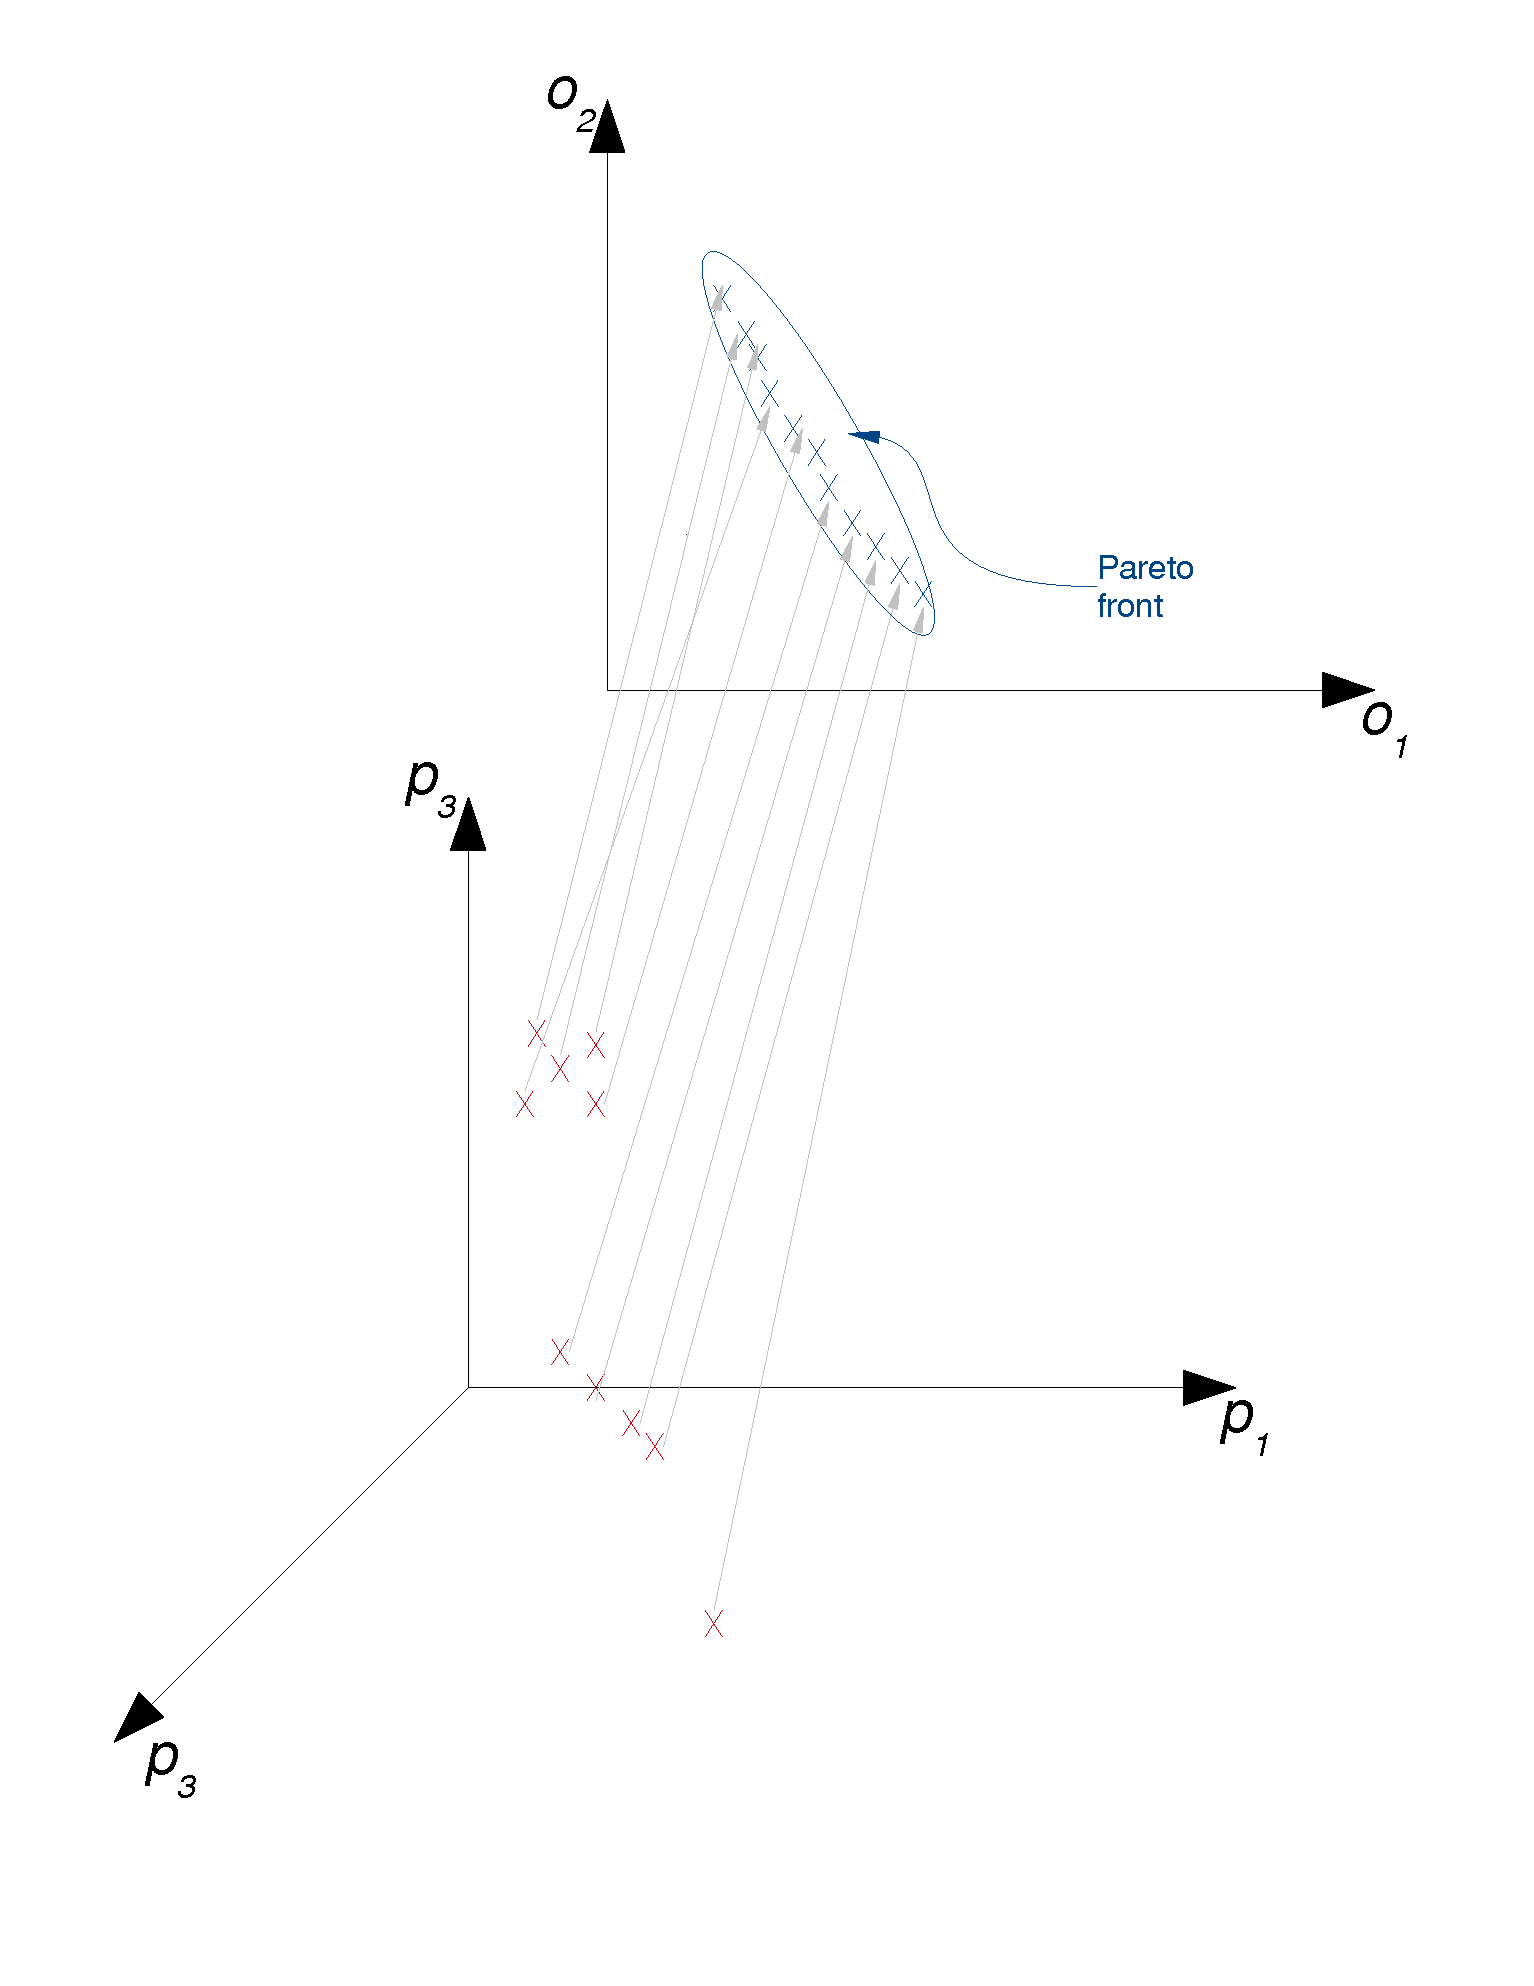
\includegraphics[width=0.5\columnwidth]{img/Pareto_set_and_front}
\caption{Relation between Pareto set (its ``parameter space representation'')
and Pareto front (``objective space representation'').}
\end{figure}

\subsection{Sketch of the Idea}
\secL{sketch}

In the design process, there are often a lot of ``local decisions''
in which the designer can take advantage of well-known results or
heuristics. For example, if we consider a VLIW architecture in a configuration with very few registers, it is well-known that increasing the number of ALUs does not bring tangible better performances
but only cause an increase in area occupation. An intelligent exploration
algorithm would not waste time evaluating configurations with many
ALUs and few registers. If $p_{1}$ is the parameter ``number of
registers'' and $p_{2}$ is the parameter ``number of ALUs'', we
can say that the region:
\[
R=\left\{ \left.\left(v_{1},v_{2}\right)\in P_{1}\times P_{2}\right|v_{1}<s_{1},v_{2}>s_{2}\right\} 
\]
 (where $s_{1}$ and $s_{2}$ are some threshold values) is \emph{uninteresting}. This clearly shows that there are cases when, if a parameter lies in
a certain range, there are ranges of the other that are not worth exploring. Intuitively, the Cartesian product of these ranges is an ``uninteresting
 region''.

The problem is that, in complex scenarios, not all relations of this
kind are known in advance. Some dependency may exist but may be hidden
to the designer. Or they may be ``local'', i.e. two
parameters may be related by a dependency but only if their values
lie on some ranges (so we cannot treat them as they were related by
a ``complete'' dependency). 
Therefore, as stated in section \ref{sec:Related-work},
setting up an exploration trying to take into account as much dependencies
as possible is a hard task that is destined to be incompletely
accomplished. We need a methodology to ``automatically'' recognize
interesting or uninteresting regions without requiring a priori knowledge
to the designer, that is what our algorithm does.

We also consider, in measuring how much interesting a region is, the
\emph{innovation} that it adds. If, during a design space exploration,
a Pareto front is temporarily calculated, adding a new Pareto front
point near to the previous ones is not a considerable innovation,
because the way it fulfills the objectives is similar to the other
already evaluated configurations. On the contrary, adding a new Pareto
front point that is distant from previous ones is remarkable,
since it let the experimenter discover potential performance that have not yet considered before.

%TODO: sync name of values with formulation
\subsection{Formal definitions}
We start by defining the parameter interval and the concept of interval contiguity. Using these definition we construct the region and define the region contiguity. Then we define the operations of splitting and merging regions. Finally, we provide the definition of separation.

\begin{definition}[Parameter Interval] Let $p_{i}$ be a parameter and $a_{i},b_{i}\in V_{i},a_{i}<b_{i}$.
A $p_{i}$- interval is
\[
\left[a_{i}..b_{i}\right]=\left[a_{i},b_{i}\right]\cap P_{i}
\]
i.e. taking the interval $\left[a_{i}..b_{i}\right]$
is the set of values of $V_{i}$ lying in $\left[a_{i},b_{i}\right]$)
\end{definition}

We consider only parameters $p_{i}$ with ordering, i.e. such
that $\forall a,b\in V_{i}$ it is possible
to say $a<b$ or $a=b$ or $a>b$.


%TODO: DESCRIVERE COME SI PENSA DI TRATTARE GLI SCENARI IN CUI ESISTONO
%PARAMETRI SENZA ORDINAMENTO{]}

	\begin{figure}[t]
		\begin{center}
			\subfigure[Examples of contiguous and non contiguous intervals.]{
				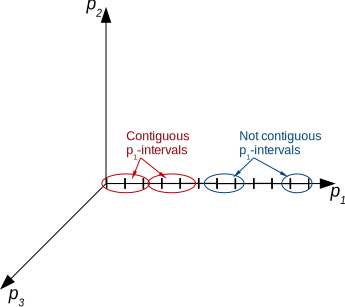
\includegraphics[width=0.45\textwidth]{img/contiguous_intervals_or_not} }
			\subfigure[Examples of regions.]{
				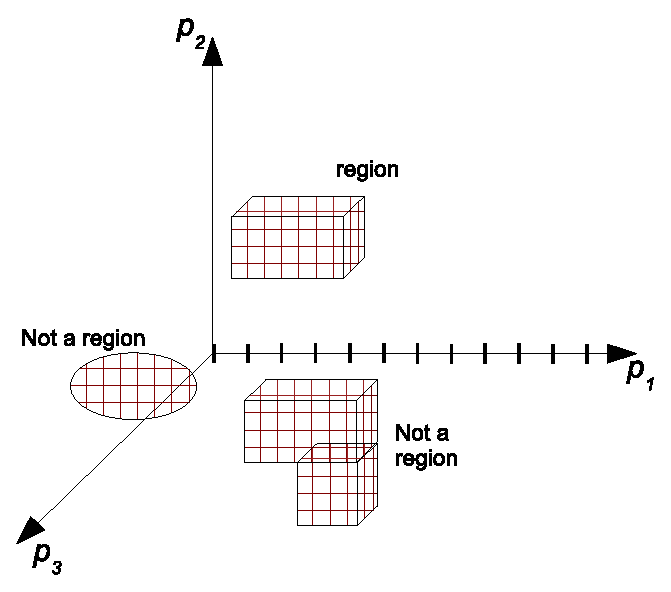
\includegraphics[width=0.45\textwidth]{img/regions} }
		    \figLC{interval_and_region}{Intervals and regions.}
		\end{center}
	\end{figure}


\begin{definition}[Contiguous intervals]
\label{pers02.def:Contiguous-intervals}
Two intervals are contiguous iff they do not overlap and merging them results in a new interval.More formally, let $\left[a_{i}..b_{i}\right]$ and $\left[x_{i}..y_{i}\right]$
be two $p_{i}$-intervals. They are said to be contiguous (see \figR{interval_and_region}(a) ) iff
\begin{align}\begin{array}{l}
	\left[a_{i}..b_{i}\right]\cap\left[x_{i}..y_{i}\right]=\emptyset \mbox{      and} \\
	\left[a_{i}..b_{i}\right]\cup\left[x_{i}..y_{i}\right]$ is a $p_{i}$-
interval or $\left[x_{i}..y_{i}\right]\cup\left[a_{i}..b_{i}\right]
\end{array}\end{align}
\end{definition}

\begin{definition}[Region] 
A region is a cartesian product of parameter intervals, as illustrated in \figR{interval_and_region} (b). More formally, if $p_1,\dots,p_n$ are the parameters of the system, and $\left[ a_{i}..b_{i} \right]$ is a $p_i$-interval, a region is a set of the following form:
\[
R=\left[a_{1}..b_{1}\right]\times\dots\times\left[a_{n}..b_{n}\right]=\prod\left[a_{i}..b_{i}\right]
\]
\end{definition}

We will refer later to ``big'' and ``small'' regions. The sense
of these terms is related to the cardinality of regions.
\begin{definition}[Interval and region comparison]
A $p_{i}$-interval $\left[a_{i}..b_{i}\right]$
is said to be bigger then another $p_{i}$-interval $\left[c_{i}..d_{i}\right]$
iff 
$\left|\left[a_{i}..b_{i}\right]\right|>\left|\left[c_{i}..d_{i}\right]\right|$.
Similarly, a region $R_{1}$ is said to be \emph{bigger }then $R_{2}$, if
$\left|R_{1}\right|>\left|R_{2}\right|$
\end{definition}
Note that with $|\cdot|$ we indicate the cardinality of a set. Therefore, $\left|\left[a_{i}..b_{i}\right]\right|$ is the number of values of $V_i$ lying between $a_{i}$ and $b_{i}$ and has not to be confused with $b_i - a_i$.
Similarly $\left|R_{i}\right|$ is the number of configurations inside the region $R_i$.

We now provide some rules to split and merge regions. They will be
useful when explaining our proposed exploration algorithm.
\begin{definition}[Splitting an interval]
\defL{splitting-a-region}
Given a $p_i$ interval $\left[a_{i}..b_{i}\right]$ with more than one element, i.e. $\left|\left[a_{i}..b_{i}\right]\right|>1$, the splitting operation produces as result two contiguous intervals $\left[a_{i}..c_{i}\right],\left[d_{i}..b_{i}\right]$
 such that
	\begin{align}
		\begin{cases}
		\left[a_{i}..c_{i}\right]\cap\left[d_{i}..b_{i}\right] & =\emptyset\\
		\left[a_{i}..c_{i}\right]\cup\left[d_{i}..b_{i}\right] & =\left[a_{i}..b_{i}\right]\\
		\left|\left[a_{i}..c_{i}\right]\right| & =\left\lceil \frac{\left|\left[a_{i}..b_{i}\right]\right|}{2}\right\rceil 
		\end{cases}
	\end{align}

We define the split operator $\psi$ as the one that, applied to the intervals, gives the result of the split operation, i.e., in the case above, $\psi \left[a_{i}..b_{i}\right]=\lbrace \left[a_{i}..c_{i}\right],\left[d_{i}..b_{i}\right] \rbrace$.
If $\left|\left[a_{i}..b_{i}\right]\right|=1$, the interval
cannot be split and $\psi \left[a_{i}..b_{i}\right]=\left[a_{i}..b_{i}\right]$.
\end{definition}

The interval split is illustrated in \figR{split}~(a). Note that, when splitting an interval, the resulting intervals must satisfy two conditions: (i) they must be contiguous and, merging them, the initial interval must be obtained; (ii) the point in which we cut the interval is not arbitrary, but it is close to the middle.

\begin{definition}[Splitting a region]
\label{pers02.def:Splitting-a-region}
Consider a region $R=\prod\left[a_{i}..b_{i}\right]$.The split operator $\psi$ divides it in a set of subregions obtained splitting each $p_i$-interval and combining the resulting subintervals with the cartesian product, as in \figR{split}~(b). Formally:
	\begin{align}
		\psi(R) = \left\{ \left.\prod\left[x_{i}..y_{i}\right]\right|\left[x_{i}..y_{i}\right]\in \psi\left[a_{i}..b_{i}\right]  \right\} 
	\end{align}

\end{definition}


	\begin{figure}[t]
		\begin{center}
			\subfigure[Splitting an interval.]{
				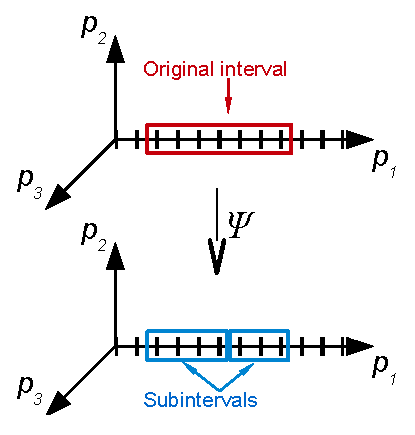
\includegraphics[width=0.30\textwidth]{img/splitting_intervals} }
			\subfigure[Splitting a region.]{
				\includegraphics[width=0.60\textwidth]{img/splitting_regions} }
		    \figLC{split}{Split operations.}
		\end{center}
	\end{figure}



\begin{definition}[Contiguous regions]Let $R_{1}=\prod\left[a_{i}\dots b_{i}\right]$ and $R_{2}=\prod\left[x_{i}..y_{i}\right]$
be two regions. They are said to be contiguous iff they do not overlap and, merging them, a new region can be obtained. Formally, $R_1$ and $R_2$ are contiguous iff there exists a $j$ such that:
	\begin{align}\begin{array}{l}
		\left[a_{i}..b_{i}\right]=\left[x_{i}..y_{i}\right]$
	\mbox{ for } $i\neq j \mbox{      and} \\
		\left[a_{j}..b_{j}\right]$ and $\left[x_{j}..y_{j}\right] \mbox{ are contiguous intervals}
	\end{array}\end{align}
\noindent We call $p_j$ the \emph{contiguity parameter} for the two regions.
\end{definition}

Examples of contiguous and non contiguous regions are given in \figR{contiguous_regions}. 
\comment{Spiegare le figure e inserire a dx una figura con le contiguous regions mergiate. Le definizioni buttate cosi' rendono difficile la lettura a chi non sa ancora dove vogliamo andare a parare. Giustifica ogni definizione prima di darla. Ad es. quando parli di splittare, spiega che quando le regioni sono interessanti noi le splittiamo cosi' da esplorarle meglio. Al contrario quando le mergiamo. Mettere una sezione del tipo "Required operations at a glance" per giustificare tutte le definizioni prima di buttarle}.

	\begin{figure}[h]
		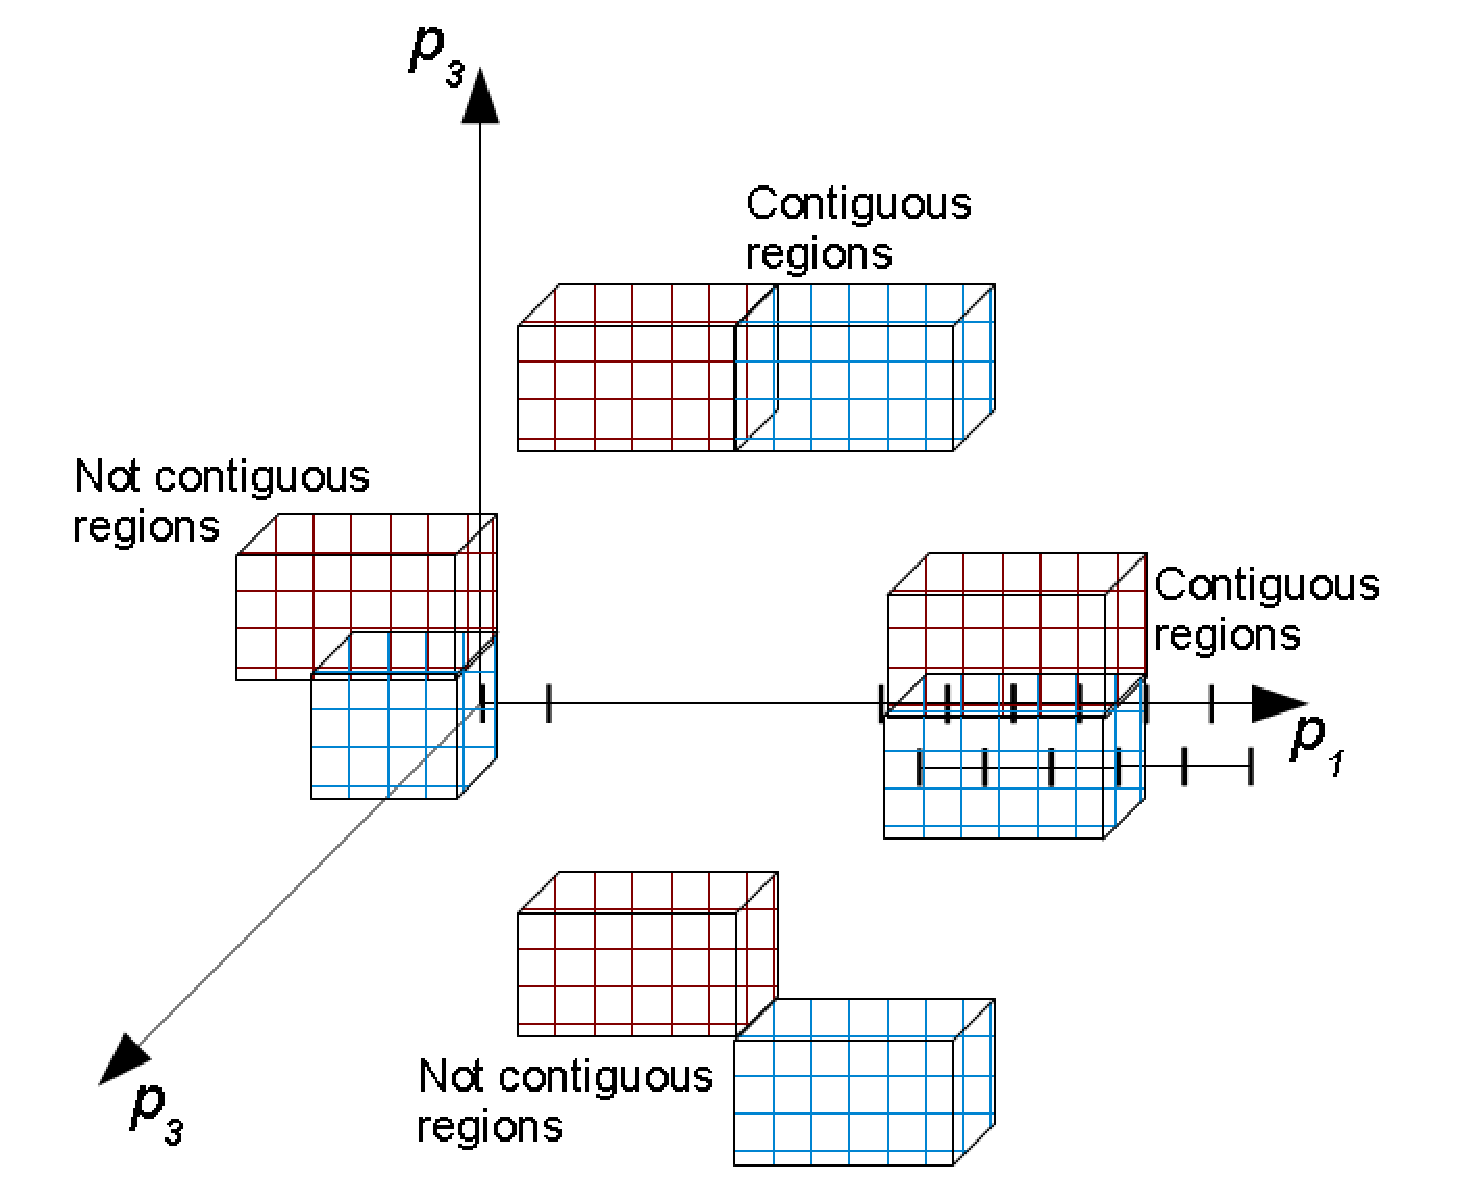
\includegraphics[width=0.5\columnwidth]{img/contiguous_regions}
		\figLC{contiguous_regions}{Contiguous and non contiguous
		regions.}
	\end{figure}


\begin{definition}[Merging intervals]
Let $\left[a_{i}\dots b_{i}\right]$ and $\left[x_{i}..y_{i}\right]$ be two contiguous $p_i$-intervals. The merge operation applied to them produces a new $p_i$-interval of the following form:
	\begin{align}
		\mu	 \left( \begin{array}{l}
				\left[a_{j}..y_{j}\right] \\
				\left[x_{j}..b_{j}\right]
		     \end{array} \right)
		=\begin{cases}
			\left[a_{j}..y_{j}\right] & \mbox{ if }b_{j}<x_{j}\\
			\left[x_{j}..b_{j}\right] & \mbox{ if }y_{j}<a_{j}
		\end{cases}
	\end{align}

\end{definition}

\begin{definition}[Merging regions]
\defL{merging-regions}
Let $R_{1}=\prod\left[a_{i}\dots b_{i}\right]$ and $R_{2}=\prod\left[x_{i}..y_{i}\right]$ be two contiguous regions and let $p_j$ be the contiguity parameter. 
The merge operation $\mu$ applied to $R_1$ and $R_2$ produces a new region of the following form:
	\begin{align}
		\mu(R_1,R_2)=\prod_{i<j}\left[a_{i}..b_{i}\right]
		\times
		\mu	 \left( \begin{array}{l}
				\left[a_{j}..y_{j}\right] \\
				\left[x_{j}..b_{j}\right]
		     \end{array} \right)
		\times
		\prod_{i>j}\left[a_{i}..b_{i}\right]
	\end{align}
\end{definition}

Note that $\mu(R_{1},R_{2})$ is mathematically equivalent to $R_{1}\cup R_{2}$. However, we use the notation above to enforce the requirement that
$R_{1}$ and $R_{2}$ must be to contiguous regions.

In \secR{sketch} we observed that, in order to estimate how much interesting is a region, it is crucial to understand the novelty that it introduces, i.e. how distant the Pareto-optimal configurations discovered in that region are from the Pareto-optimal configuration previously discovered. The concept of distance is expressed by the operator defined in the next definition. We prefer to call it \emph{separation} rather than \emph{distance}, because usually distance denote a commutative operator while our definition of separation is non commutative.

\begin{definition}[Separation]
\defL{separation}
Let $\mathbf{c}',\mathbf{c}''\in \mathcal{C}^*(S)$ be two configurations of the system $S$, $b\in\mathcal{B}$ a benchmark application and $\mathbf{o}',\mathbf{o}''\in \Re^m$ the representation of the configurations in the objective space, i.e. $\mathbf{o}'=E \left(\mathbf{c}', b\right)$, $\mathbf{o}''=E \left(\mathbf{c}'', b\right)$, where $E$ is the evaluation function. The separation between
$\mathbf{c}'$ and $\mathbf{c}''$ is 
	\[
	s\left(\mathbf{c}'\rightarrow\mathbf{c}''\right)=\sum_{i=1}^{m}\left|\frac{o'_{i}-o''_{i}}{o'_{i}}\right|
	\]
where $o'_i$ and $o''_i$ are the $i$-th components of $\mathbf{o}'$ and $\mathbf{o}''$, respectively.
\end{definition}

The separation between $\mathbf{c}'$ and $\mathbf{c}''$ measures how
much we must vary the image of the former to obtain the image of the latter. Note that the separation is a \emph{normalized} measure, thanks to $o'_i$ at the denominator. This is important since usually objectives are heterogeneous, e.g. delay and power consumption, having different unity of measurement and different scale. If we did not use a normalized measure, in presence of objectives whose absolute values are small and other objectives with big values, the notion of distance would have been biased toward the latter.


\section{PS algorithm}
\secL{algorithm}
In this section we present PS, the algorithm that we propose to perform the Design Space Exploration (DSE). As any other DSE algorithm, its input is the parametrized system $S$ and a benchmark application $b$, while the output is an approximation of the Pareto-optimal set $\mathcal{P}\left(S,b\right)$.   
PS is iterative and we will describe, separately, the initialization phase, the operations performed inside each iteration and the condition that triggers the termination.

At a glance, at each iteration simulations are performed. Regions are classified based on the innovation introduced by their configurations in the Pareto-front so far calculated. The most interesting regions are split, so that each sub-region will receive more evaluation effort in the next iteration. On the contrary, uninteresting regions are merged.

By a slightly abuse of notation, considering a subset $I$ of the configuration space, we will use  $\mathcal{P}(I,b)$ to denote the non-dominated feasible configurations in $I$, i.e.
	\begin{align}
		\mathcal{P}(I,b)=
		\left\{ \mathbf{c} \in I \cap \mathcal{C}^*(S) | \nexists \ \mathbf{c}' \in I \cap \mathcal{C}^*(S), \mathbf{c}' \succ \mathbf{c} \right\}
	\end{align}
Since in each run of the algorithm we will consider only one benchmark application $b\in\mathcal{B}$, we will omit it, replacing, for example, $\mathcal{P}(I,b)$ with  $\mathcal{P}(I)$.

Each iteration is called \emph{era}. The $i$-th era is characterized by: 
	\begin{itemize}
	\item the set of regions $\mathcal{R}_{i}$ in which the configuration space
	$\mathcal{C}(S)=V_{1}\times\dots\times V_{n}$ is partitioned
	\item an approximation $\mathscr{P}_{i}$ of the Pareto-optimal set.
	\item a set $test_{i}$ of at most $K$ configurations evaluated
	in the era.
	\end{itemize}
$K$ is a parameter that must be set before the algorithm runs.
Note that $\mathcal{R}_{i}$ is a partition of the configuration space, i.e.
	\begin{align}\begin{array}{l}
		\bigcup_{R\in\mathcal{R}_i} R = \mathcal{C}(S) \mbox{ and}\\
		R' \cap R'' = \emptyset, \forall R',R'' \in \mathcal{R}_i
	\end{array}\end{align}

We now formally describe PS.

\subsection{Initialization}
We fix $\mathcal{R}_0$, $\mathscr{P}_0$ and $test_0$ for the era $0$ as follows. Era $0$ has only one region that is the whole parameter space,
i.e. $\mathcal{R}_{0}=\left\{ V_{1}\times\dots\times V_{n}\right\} $.
A random set $test_{0}$ of $K$ configurations is evaluated. The
Pareto set $\mathscr{P}_{0}=\mathscr{P}\left(test_{0}\right)$ is
calculated.



\subsection{Iteration steps}
\secL{steps}

For $era_{i}$ with $i>0$ the following operations must be performed.
\begin{enumerate}
\item \label{pers02.enu:K}
In each era $i$, a set $test_i$ of $K$ configurations will be evaluated. We call them \emph{test configurations} and selecting them is exactly the goal of this step.
We select only \emph{new} configurations, i.e. the ones that have not been evaluated in past eras. In other words, $test_i$ must not overlap with $\bigcup_{j=0}^{i-1}test_{j}$.
Since all regions $R$ in the configuration space partition $\mathcal{R}_{i}$ must be properly explored, we have to distribute the test configurations among all these regions. For this reason, $\frac{K}{\left|\mathcal{R}_{i}\right|}$ configurations are randomly extracted from the new configurations of each region $R\in\mathcal{R}_{i}$. We use $test_{R,i}$ to denote the set of the selected configurations and, obviously, $\bigcup_{R\in\mathcal{R}_{i}} test_{R,i} = test_i$.
 In case the new configurations in $R$ are less then $\frac{K}{\left|\mathcal{R}_{i}\right|}$, all of them are selected. In this case $test_{R,i}=R\setminus\bigcup_{j=0}^{i-1}test_{j}$, where  $\bigcup_{j=0}^{i-1}test_{j}$ is the set of the configurations already evaluated in the past.\footnote{Note that if such regions exist, the total number of evaluations in era $i$ will be less than $K$}
\item All configurations on $test_{i}$ are simulated.
\item The Pareto set $\mathscr{P}_{i}$ for $era_{i}$ is defined as the set of non-dominated configurations among the ones evaluated so far, i.e.
	\[
	\mathscr{P}_{i} \triangleq
	\mathscr{P}\left(\bigcup_{j\leq i}test_j\right)=
	\mathscr{P}\left(test_{i}\cup\mathscr{P}_{i-1}\right)
	\]
where the last equality can easily be proved.

\item \label{pers02.enu:novelty_score_of_a_configuration}
The test configurations that are dominated, i.e. do not belong to $\mathscr{P}_i$, are neglected, while an \emph{innovation score} is given to the other ones, computed on the base of their separation from the non-dominated configurations of the past eras. Recalling that $s$ is the separation (see \defR{separation}), the innovation score of a non-dominated test configuration $\mathbf{c}^*$ is defined as
	\[
	is\left(\mathbf{c}^*\right)=\min\left\{ \left.s\left(\mathbf{c}^*\rightarrow\mathbf{c} \right)\right|\mathbf{c}\in\mathscr{P}_{i-1}\right\} 
	\]
In other words, a configuration $\mathbf{c}^*$ is characterized by as much innovation
as more separated it is from the configurations of the previous era.

\item \label{enu:region_innovation_score} Every region $R\in\mathcal{R}_{i}$ is given an innovation score defined
as the sum of the innovation scores of its non-dominated test configurations:
	\[
	is\left(R\right)=\sum\left\{ \left.is\left(\mathbf{c}\right)\right|\mathbf{c}\in\mathscr{P}_{i}\cap test_{R,i} \right\} 
	\]

\item The total innovation and average score for the entire era is calculated:
	\begin{align} \begin{array}{l}
	is_{TOT,i}=\sum_{R\in\mathcal{R}_{i}}is\left(R\right) \\
	is_{av,i}=is_{TOT,i} / |\mathcal{R}_i|
	\end{array} \end{align}
	

\item The configuration space partition $\mathcal{R}_{i}$ is divided in three subsets, that we will comment later:

	\begin{enumerate}
	\item \emph{high innovation regions}, whose innovation score exceeds the average score of the previous era by a factor of $\alpha$, i.e.
	\[
	\mathcal{R}_{i,h}=\left\{ \left.R\in\mathcal{R}_{i}\right|is\left(R\right)>\alpha\cdot is_{av,i-1}\right\} 
	\]
	 where $\alpha$ is a constant defined by the designer (for example
	$\alpha=1.2$). 	
	\item \emph{low innovation regions}, whose score is positive but modest, i.e.
	\[
	\mathcal{R}_{i,l}=\left\{ \left.R\in\mathcal{R}_{i}\right|0<is\left(R\right)\le\alpha\cdot is_{av,i-1}\right\} 
	\]
	\item \emph{no innovation regions}, whose innovation is null, i.e. 
	\[
	\mathcal{R}_{i,n}=\left\{ \left.R\in\mathcal{R}_{i}\right|is\left(R\right)=0\right\} 
	\]
	\end{enumerate}

\item The goal of this step is preparing the regions that will compose the configuration space partition of the next era, i.e. $\mathscr{R}_{i+1}$. The following operations are performed:
	\begin{enumerate}
		\item Each high innovation region $R\in\mathscr{R}_{i,h}$ is split to obtain $\psi(R)$, as stated in \defR{splitting-regions}. We use $\psi\left(\mathscr{R}_{i,h}\right)$ to denote the set of regions obtained as explained.
		\item Low innovation regions are left unchanged.
		\item No innovation regions are merged, two by two. To do so, pairs of no innovation contiguous regions $(R_1,R_2)$ are selected. We use $\mathscr{M}_i$ to represent the set of these pairs. This set is constructed such that pairs are independent, i.e. there cannot be two of them sharing a region. In other words, taking whatever $(R_1,R_2),(R_3,R_4) \in \mathscr{M}_i$, $R_i \neq R_j, \forall i,j\in\lbrace1,2,3,4\rbrace, i\neq j$. 
We merge each pair of these regions, i.e. $\forall (R_1,R_2)\in\mathscr{M}_i$ we calculate $\mu(R_1,R_2)$, according to \defR{merging-regions}.
We stress that the regions that belong to each selected pair must be contiguous, otherwise it is impossible to merge them. We use $\mu(\mathscr{M}_i)$ to denote the set of the merged regions, i.e. $\mu(\mathscr{M}_i) = \bigcup_{(R_1,R_2)\in\mathscr{M}_i} \mu(R_1,R_2)$
	\end{enumerate}


\item The set of regions $\mathcal{R}_{i+1}$ for the following era is composed of the sub-regions resulting from splitting operations ($\psi\left(\mathscr{R}_{i,h}\right)$), the low innovation regions unchanged $\mathcal{R}_{i,l}$, the result of the merging operations ($\mu(\mathscr{M}_i))$ and the no innovation regions that was not possible to merge $\left(\mathcal{R}_{i,n}\setminus\bigcup_{\left(R_{1},R_{2}\right)\in\mathscr{M}_i }\left\{ R_{1},R_{2}\right\} \right)$. Formally:
	\begin{align} 
	\mathcal{R}_{i+1} \triangleq
	\psi\left(\mathscr{R}_{i,h}\right) \cup \mathcal{R}_{i,l}\cup
	\left(\mathcal{R}_{i,n}\setminus\bigcup_{\left(R_{1},R_{2}\right)\in\mathscr{M}_i }\left\{ R_{1},R_{2}\right\} \right)\cup \mu(\mathscr{M}_i)
	\end{align}
\end{enumerate}

\begin{algorithm}[t]
	\small
	\caption{PS Algorithm}
	\label{alg:algo}
	  \SetKwInOut{Input}{Input}\SetKwInOut{Output}{Output}
	  \Input{S}
	  \Output{ $\tilde{\mathscr{P}}$ // Approximation of Pareto-set}
%
	  \nl //Initialization \\
	  \nl $\mathscr{R}_0\Leftarrow
				\left\{ V_{1}\times\dots\times V_{n}\right\} $; \\
	  \nl $\mathscr{P}_0\Leftarrow $ extract\_non\_dominated($test_0$);\\
	  \nl \\
	  \nl $i\Leftarrow 0$;\\
	  \nl \While{ !termination\_condition } {
			// Iteration steps\\
			\nl $test_i=\emptyset$;\\
	  		\nl \ForEach {$R \in \mathscr{R}_i$}{
				\nl $\mathscr{N}_{R,i} \Leftarrow$ configurations in $R$ not evaluated so far;\\
				\nl $|\mathscr{N}_{R,i}|\leq K/|\mathscr{R}_i|$? \\
						$\mbox{\,\,\,\,\,\,\,\,\,\,\,\,\,\,\,\,\,\,}test_{R,i}\Leftarrow \mathscr{N}_{R,i}$:\\
						\mbox{\,\,\,\,\,\,\,\,\,\,\,\,\,\,\,\,\,\,}$test_{R,i}\Leftarrow K/|\mathscr{R}_i|$ randomly selected configurations from $\mathscr{N}_{R,i}$;\\
			\nl $test_i\Leftarrow test_i \cup test_{R,i}$

			}

			\nl simulate ($test_i$);\\
			\nl $\mathscr{P}_i \Leftarrow 
				\mathscr{P}\left(test_{i}\cup\mathscr{P}_{i-1}\right)$;\\
			\nl \ForEach{$\mathbf{c}^*\in\mathscr{P}_i$} {
				\nl $is\left(\mathbf{c}^*\right) \Leftarrow \min\left\{ \left.s\left(\mathbf{c}\rightarrow\mathbf{c} \right)\right|\mathbf{c}\in\mathscr{P}_{i-1}\right\}$;\\
				}
			\nl \ForEach{$R\in\mathscr{R}_i$} {
				\nl $is\left(R\right)=\sum\left\{ \left.is\left(\mathbf{c}\right)\right|\mathbf{c}\in\mathscr{P}_{i}\cap test_{R,i} \right\} $;
			}

			\nl $is_{TOT,i}=\sum_{R\in\mathcal{R}_{i}}is\left(R\right)$ \\
			\nl $is_{av,i}=is_{TOT,i} / |\mathcal{R}_i|$\\
			\nl \\ //Region classification\\
			\nl $\mathcal{R}_{i,h}=\left\{ \left.R\in\mathcal{R}_{i}\right|is\left(R\right)>\alpha\cdot is_{av,i-1}\right\}$; \\
			\nl $\mathcal{R}_{i,l}=\left\{ \left.R\in\mathcal{R}_{i}\right|0<is\left(R\right)\le\alpha\cdot is_{av,i-1}\right\} $; \\
			\nl $\mathcal{R}_{i,n}=\left\{ \left.R\in\mathcal{R}_{i}\right|is\left(R\right)=0\right\} $;
			
			\nl \\ // Splitting and merging operations\\
			\nl $\psi(\mathscr{R}_{i,h}) \Leftarrow \lbrace 
					\psi(R) | R\in \mathscr{R}_{i,h}	
				\rbrace$; \\
			\nl construct $\mathscr{M}_i$; // the set of pair of contiguous no innovation regions \\
			\nl $\mu(\mathscr{M}_i) = \bigcup_{(R_1,R_2)\in\mathscr{M}_i} \mu(R_1,R_2)$;\\
			\nl\\ // Prepare the configuration space partition for the next iteration \\
			\nl $\mathcal{R}_{i+1} \triangleq
	\psi\left(\mathscr{R}_{i,h}\right) \cup \mathcal{R}_{i,l}\cup
	\left(\mathcal{R}_{i,n}\setminus\bigcup_{\left(R_{1},R_{2}\right)\in\mathscr{M}_i }\left\{ R_{1},R_{2}\right\} \right)\cup \mu(\mathscr{M}_i)$;\\
		}
	\nl $\tilde{\mathscr{P}} \Leftarrow \mathscr{P}_i$
\end{algorithm}

\subsection{Termination Condition}
The algorithm terminates at step $k$ if
\[
is_{TOT,k},is_{TOT,k-1},\dots,is_{TOT,k-\beta}\le\gamma\cdot is_{TOT,k-\left(\beta-1\right)}
\]
 where $\beta$ and $\gamma$ are selected by the experimenter. 
In other words, the algorithm terminates if, in the last
$\beta$ iterations, the ``amount of innovation'' has been
small. Therefore, it is very probably that carrying on iterating
will not considerably change the Pareto-front approximation already formed. 

It is not recommended to chose $\beta=1$, because it is possible that the
$k-1$-th and $k$-th Pareto front approximations are not very different but next ones could be. In other words,
it is unsafe to terminate as soon as the Pareto front does not considerably change
between two consecutive eras. For this reason, we take into
account the history of the Pareto fronts.

A pseudo-code representation of PS algorithm is in Alg.\ref{alg:algo}.
%!!! IN INGLESE E' PIU' CORRETTO DIRE: ``IT IS POSSIBLE THAT THE PARETO
%FRONTS WERE NOT VERY DIFFERENT''? (CON ``WERE'' AL POSTO DI ``ARE'')

\subsection{Exploration vs. Exploitation in PS}
The proposed algorithm has been designed in order to be inherently able to balance exploration and exploitation, which are ``two cornerstones of problem solving by search''~\cite{eiben1998evolutionary}. While a detailed survey on the exploration vs. exploitation trade-off can be found in~\cite{vcrepinvsek2013exploration}, here we limitedly recall that \emph{exploration} is the capability of an algorithm to consider different parts of the configuration space, not being confined only to a limited subset, and thus not being trapped in local optima. Following the terminology of \cite{weise2012evolutionary}, if the exploration is not sufficiently wide, the algorithm suffers from \emph{premature convergence}, i.e. it starts to analyze only a narrow portion of the configuration space, thus ignoring potential Pareto configurations that are outside this portion. When premature convergence happens, there is insufficient \emph{diversity}~\cite{weise2012evolutionary}, i.e. all the provided solutions are similar.
On the other hand, \emph{exploitation} is the capability to recognize and densely analyze the parts of configuration space that have many Pareto configurations.

While in genetic algorithms exploration and exploitation are guaranteed by mutation, crossover and selection, in our algorithm these guarantees are provided for the following reasons:
	\begin{itemize}
		\item Merging and splitting operations are dynamic processes. A portion
of the parameter space may be populated by a large number of small
regions in some eras, and thus a large number of test configurations. However, after having been sufficiently explored, the innovation score of these regions may decrease, they may be merged and therefore that portion of configuration space may be covered by a small number of large regions in next eras. This is a desirable property of PS, since, after a number of eras of intense exploration of a configuration space part, this exploration may turn out to be enough thorough and so it may be time for other parts to be minutely scanned. 
PS dynamics can be summarized as follows: while eras alternate, PS zooms out from the configurations subspaces already sufficiently scanned in the past, whereas it zooms in on subspaces which provide novelty (guaranteeing exploitation), meaning that they have not been properly analyzed yet (this helps exploration). 
		\item No portion of parameter space is neglected since, at each era, all the regions, even the least interesting ones, have the chance to be explored with new evaluated points (providing exploration), even though some regions are less densely explored than others.
	\end{itemize}

To summarize, thanks to the above characteristics, PS is able to recognize the regions where the best configurations are, while avoiding premature convergence, not being trapped in a narrow subset of configuration space.

%

\subsection{Algorithm Parameters and Scalability} The parameters that determine the algorithm are the configurations budget for each
era $K$ and the threshold factor $\alpha$. From a functional point of
view, $K$ is somewhat similar to the population size of a genetic
approach, determining how many configurations should be evaluated in the
subsequent step of the algorithm. However, as seen in the
previous subsection, the way this $K$ configurations are distributed
across the parameters space is completely different.
Authors of \cite{zitzler_ec00} found that
increasing $K$ not necessarily has a considerable impact on the
performance of the algorithm, and this holds also in our algorithm (see for example
Figure~\ref{fig:kimpact} and Subsection~\ref{sec:comparison}).
Nonetheless, while in the genetic approach $K$ must be sufficiently large
in order to guarantee the diversity of the Pareto set configurations, in
our algorithm the diversity is not impacted by $K$ since, by
construction, it is guaranteed by the way the configuration space is
partitioned, independently of the number of configurations evaluated at
each iteration. 

On the other side, parameter $\alpha$ determines when a region is considered of high
innovation. High values of $\alpha$ mean that a region will hardly be
elected as high-innovation, producing less splitting operations. This
slows down zooming in on portions of configuration space and makes the
distribution of the simulated configurations more uniform, since there are
fewer small regions with a high test configuration concentration. The
opposite happens when small values of $\alpha$ are used. In this
introductory work we are not explicitly focused on investigating how
these parameters could be fine tuned, nevertheless
we conducted some preliminary tests to confirm the relative stability
of $PS$ with different choices and to select some ``reasonable'' average
values to perform the design space exploration, as we will discuss
in~\secR{ee}.

With regard to the performance of the proposed approach, we observe it is related to the total number of
different configurations evaluated during the exploration. We can
safely make such assumption, because the process of evaluating a new
configuration is the time-dominating one among all the operations
performed. As we will show in the
next Section, this is especially true in the hardware/software
design space exploration scenario we are addressing, since benchmark
compilation and execution times
are orders of magnitude bigger than the splitting/merging operations and
innovation scores computations.  The $i$-th era would provide a new set
$test_i$ of $K$ configurations to be tested. However, we cannot know
a priori how many of
these will actually be new configurations, i.e. requiring a process of
evaluation. Thus, the number of total new simulations $N_{tot}$ 
is bounded as follows:
\[
K \le N_{tot} \le K \times E_{tot}
\]
where $E_{tot}$ is the number of eras executed and assuming that at
least $K$ evaluation should be performed in order to obtain the first
Pareto $\mathscr{P}_0$. 


\subsection{On the parallelizability of PS}
While the detailed analysis and the evaluation of a parallel
implementation of the proposed algorithm is not in the scope of this paper, we
provide in this subsection some arguments to show different strategies
that could be applied to make PS execution parallelizable.

Following the approach used in the ``Master-Slaves parallel genetic
algorithms''~\cite{Cantu-Paz98asurvey,Borkar14parallel}, we can
distinguish a master and different slave processing nodes. At each era
the master assigns a set of regions to each slave, which, in turn,
independently performs the analysis and calculates the innovation
score of the assigned regions. At the end of each era, the master
collects the results from the slaves, performs the splitting/merging
operations and the next era starts.

Another possible approach is closer to the ``Island scheme'' for GA
parallelization~\cite{Borkar14parallel}. The configuration space is
initially divided in $n$ macro-regions, each one assigned to a
different processing node, which autonomously performs all the PS
steps. When merging and splitting, each processing node consider the assigned
macro-region as the entire parameter space. Note that, while the
Island scheme for GA parallelization requires a migration operator,
that is not easy to properly tune, we do not have special
requirements. On the other hand, one of the macro-regions may begin to
provide very low innovation at a certain era. In this case, dedicating
to it the same number $K$ of test functions as to the other macro-regions
is inefficient. To solve this problem, the number of test functions
assigned to each macro-region should be periodically renegotiated, in
favor of the macro-regions providing most innovation.

Opposite to the ``Island  scheme'', a novel parallelization technique
permitted by PS can consist of different instances of PS, each one
running on the whole configuration space but having its own
configuration space partition that separately evolves. Each PS
instance independently performs the zoom-out and zoom-in on
configuration space, splitting and merging its own regions. All PS
instances share the indication of the configurations already tested,
so that a configuration already tested by some PS instance, will not
be tested again by some other PS instance. In addition, PS instances
share the set of non-dominated configurations. Therefore, when a PS
instance evaluates the innovation score of its regions (steps
\ref{pers02.enu:novelty_score_of_a_configuration} and
\ref{enu:region_innovation_score} of \secR{steps}), it considers also the
solutions found by the other PS instances. In this way, the
configuration space is spanned in parallel by multiple PS instances,
that, although autonomous, are not isolated; on the contrary, they
continuously exchange information and influence each other, thanks to
the sharing of the the set of already simulated configurations and the set of non-dominated
ones. Otherwise stated, all the PS instances (independently but
jointly) contribute to the formation of the Pareto-set.

We defer the evaluation of these different proposals to our future
research, the aim of this section being just to show that our
algorithm has the potentiality of being parallelized, thus leaving
room for performance improvement.

\section{A Case Study: VLIW Hardware/Software Design Space}
\label{sec:ee}
In order to evaluate the behavior of the proposed approach
we will be using a parameterized Very Long Instruction
Word (VLIW) architecture~\cite{kathail_tr00} as testbed. The same philosophy
behind a VLIW system makes this a natural choice for several reasons:
\begin{itemize}
\item{Multi-Objective trade-offs}: VLIW architectures let designers
easily trade between power, energy and performances~\cite{}, leading
to Pareto sets whose extension is an ideal ground for our testing
purposes focused on parameter-space space representation of Paretos.
\item{Compiler awareness}: Instruction Level Parallelism (ILP)
constitutes the key feature to enable the multi-objective trade offs
of the point above. It is statically obtained by the compiler which
performs code trasformations being aware of the underlying hardware
configuration.  This tight hardware/software dependence, makes the
VLIW scenario well suitable for investigating hardly predictable
hardware/software interactions, especially when compared to
architectures that, in order to preserve binary compatibility,
separate software generation processes from the hardware that
will execute it.

System parameters can be classified in three main categories:
\emph{processor}, \emph{memory sub-system} and \emph{compiler}. 
The first is directly related to the VLIW core and includes the size
of the register files and the number of functional
units for each type. In particular, five different types of register
files are supported:
GPR (32-bit registers for integers), FPR (64-bit registers for
floating point values) PR (1-bit registers used to store the Boolean
values of predicated instructions), BTR (64-bit registers containing
information about possible future branches) and CR (32-bit control
registers containing information about the internal state of the
processor). The functional units involved are: \emph{Integer units},
\emph{floating point units}, \emph{memory units} (associated with
load/store operations) and \emph{branch units} (associated with branch
operations). With respect to the memory sub-system, the parameters
include \emph{size}, \emph{associativity} and
\emph{block size} for each of the three caches: First-level data cache
(L1D), first-level instruction cache (L1I) and second-level unified
cache (L2U).

Next, a set of the most impacting code compilation parameters has been
selected and included in the configuration space:
\begin{itemize}
\item{tcc\_region}: Specifies the scope of action of the compiler and the type
of code transformation involved (basic block, super block and hyper
block) 
\item {max\_unroll\_allowed}: The number of unroll iterations allowed
\item{regroup\_only}: Avoids inlining 
\item{do\_classic\_opti}: A set of classical optimization, not VLIW related,
such as common expression removal 
\item{do\_prepass\_scalar\_scheduling}: Performs a schedule before
forming regions 
\item{do\_postpass\_scalar\_scheduling}: Performs a schedule after the region formation 
do\_modulo\_scheduling  Modular scheduling 
\item{memvr\_profiled}: Performs a memory-dependencies profiling 
\end{itemize}

\subsection{Evaluation Metrics}

The results presented in the next section compare PS against a widely
adpted Multi-objective Genetic Algorithm~\cite{}. At best of our
knowledge, genetic approaches
still represent the best compromise between efficiency (i.e. time
required for exploration) and accuracy of the reported Paret Sets.
Note that for the reasons described above, mono-objective approaches have been
explicitly excluded from this analysis. Same decision has been taken
for other approaches (e.g. dependecy based~\cite{dep}) that make use of some a-priori knowledge about the
role and meaning of each parameter, since our
aim is evaluate the capacity of focusing on interesting
parameter regions without any external judgement or help based on
euristics.  Finally, it should be pointed
out that in this introductory work we will explicitly use the TODO
variant of MOGA, remainding to works like~\cite{} for a detailed
analysis on how it differs and what could be expected from similar multi-objective strategies.

The class of benchmark being considered is representative of some common
frequently running application kernels in an embedded multimedia
environment. Table~\ref{tab:bench} shows the set of applications
chosen along with a brief description.
\begin{table}
	\centering
	\caption{Benchmarks}
	\label{tab:bench}
	\begin{tabular}{ll}
	\hline
	\multicolumn{1}{c}{Benchmark} & \multicolumn{1}{c}{Application} \\
	\hline
	Alloca\_test & Memory array allocation test \\
	Bmm & Matrices multiplication and elements sum \\
	Fir\_int & Finite impulse response \\
	Mm & Floating point matrices multiplication \\
	Sha256 & Cryptocurrency header Hashing \\
	Wave & Wavefront computation \\
	\hline
	\end{tabular}
\end{table}
%------------------------------------------------------------------------------

\subsection{Results}

Set of Figures~\ref{fig:pareto_fronts_100}
and~\ref{fig:pareto_fronts_500} show the resultig pareto fronts for two
different scenarios of 100 and 500 simulations budget.

\begin{table*}
  \centering
  \begin{tabular}{ccc}
    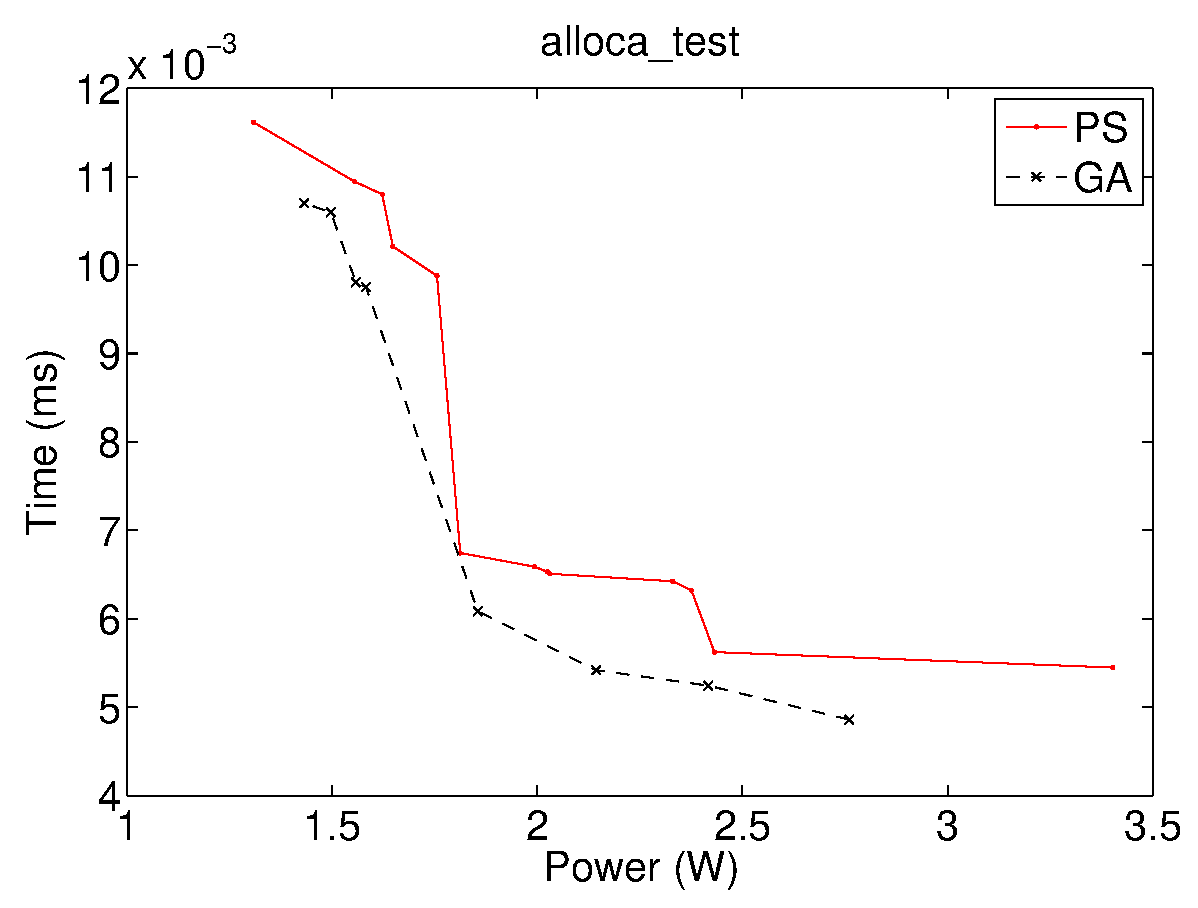
\includegraphics[width=0.30\textwidth]{pictures/alloca_100.eps} &
    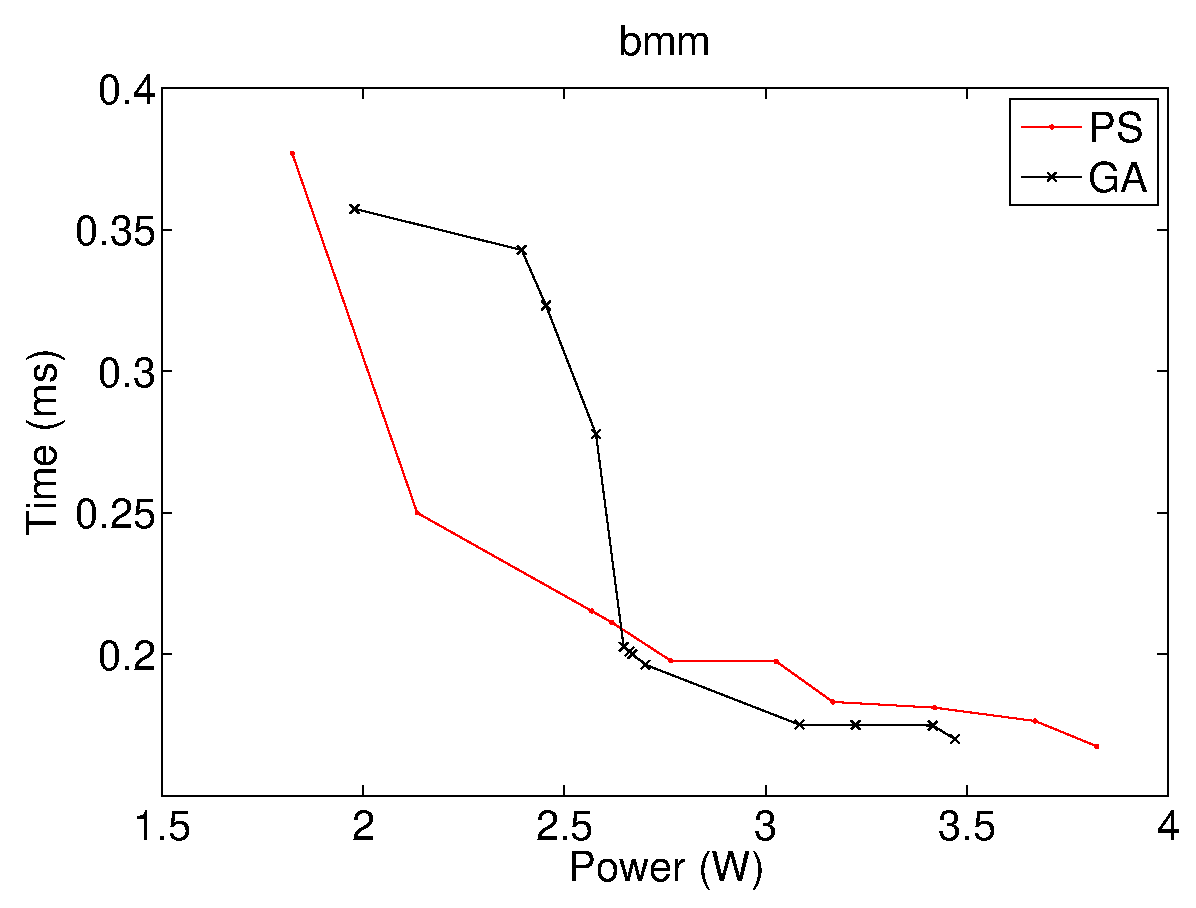
\includegraphics[width=0.30\textwidth]{pictures/bmm_100.eps} & 
    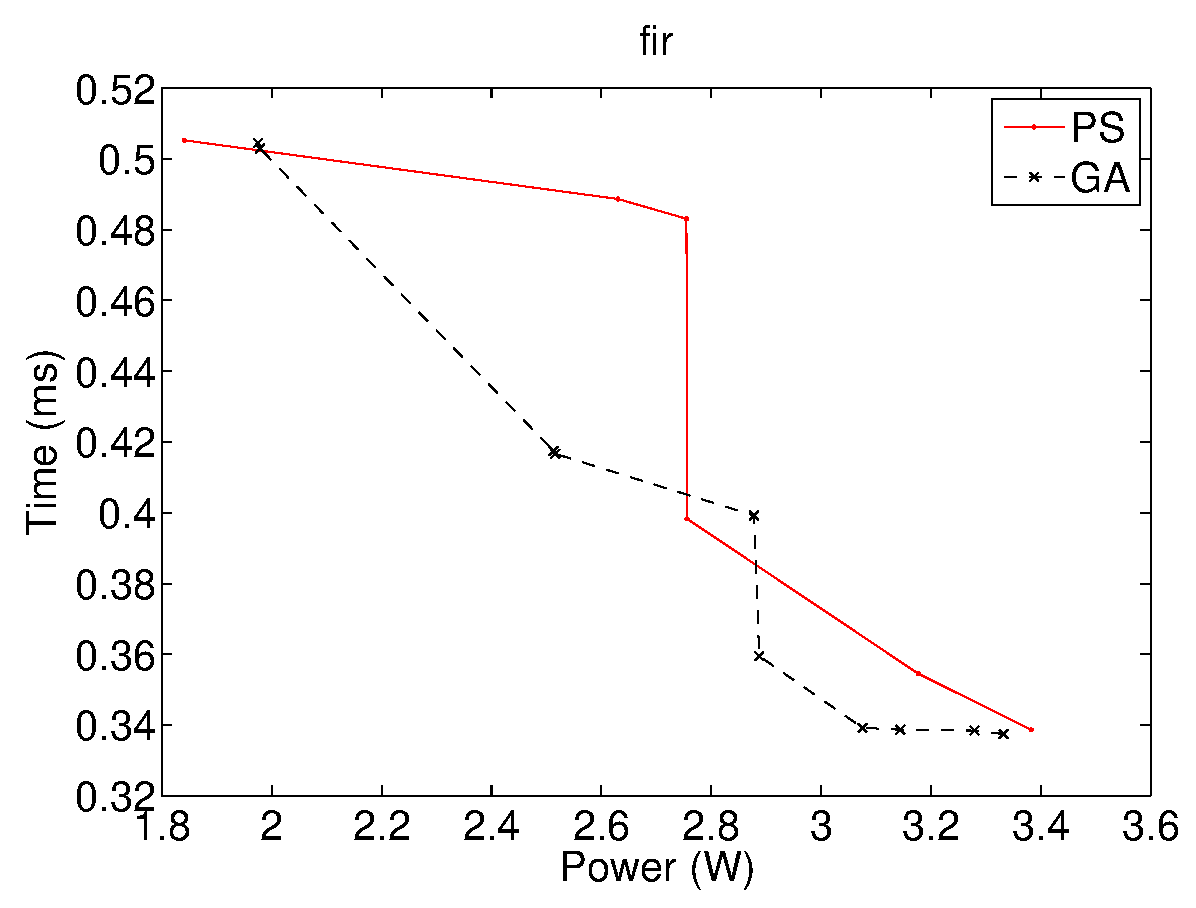
\includegraphics[width=0.30\textwidth]{pictures/fir_int100.eps} \\
    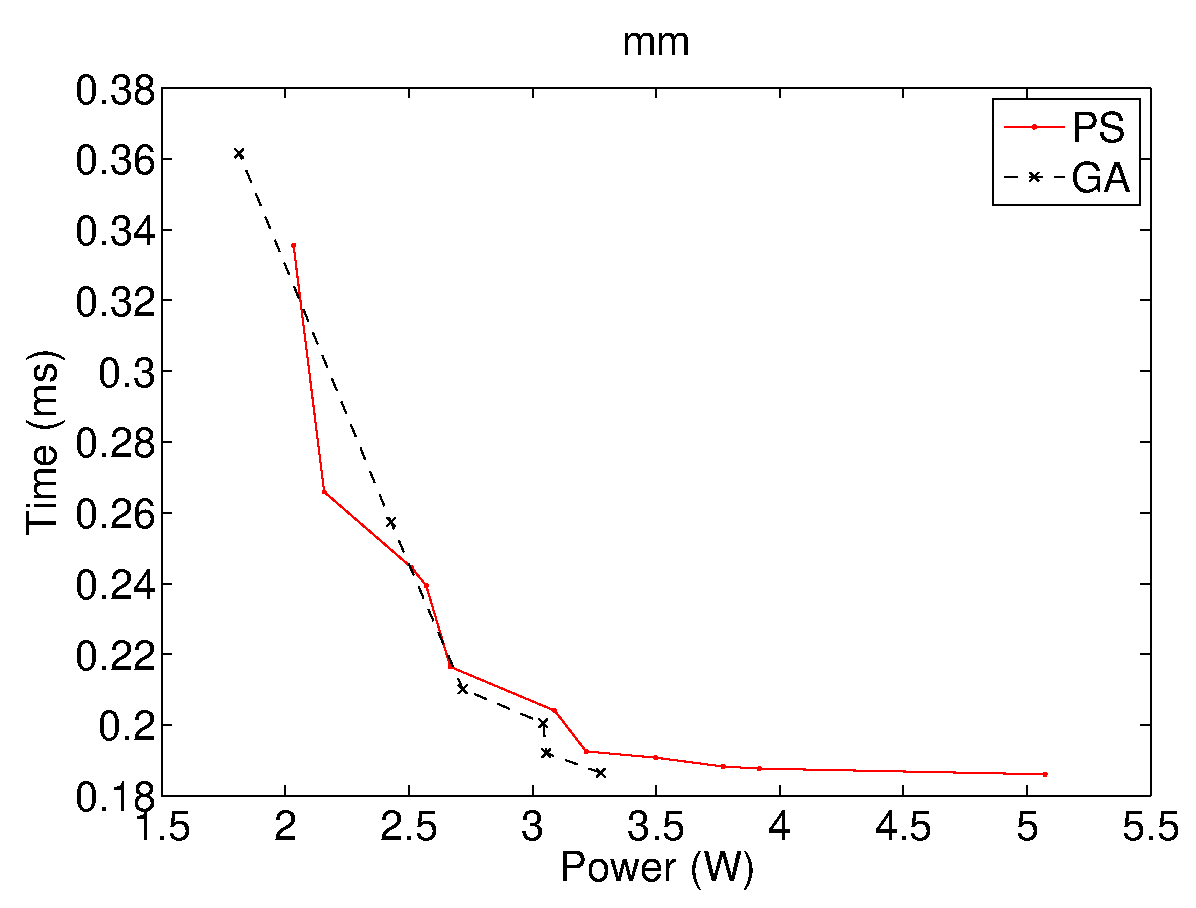
\includegraphics[width=0.30\textwidth]{pictures/mm_100.eps} &
    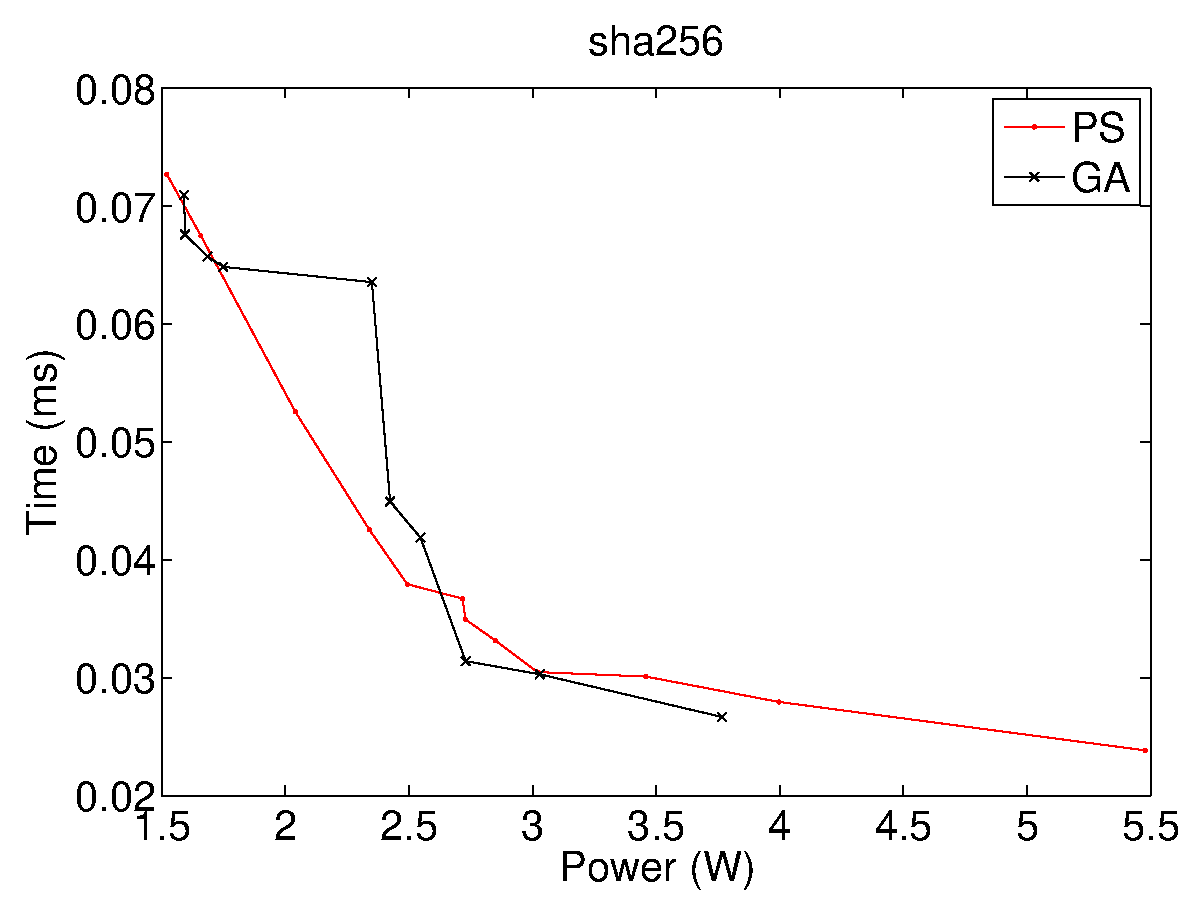
\includegraphics[width=0.30\textwidth]{pictures/sha_100.eps} &
    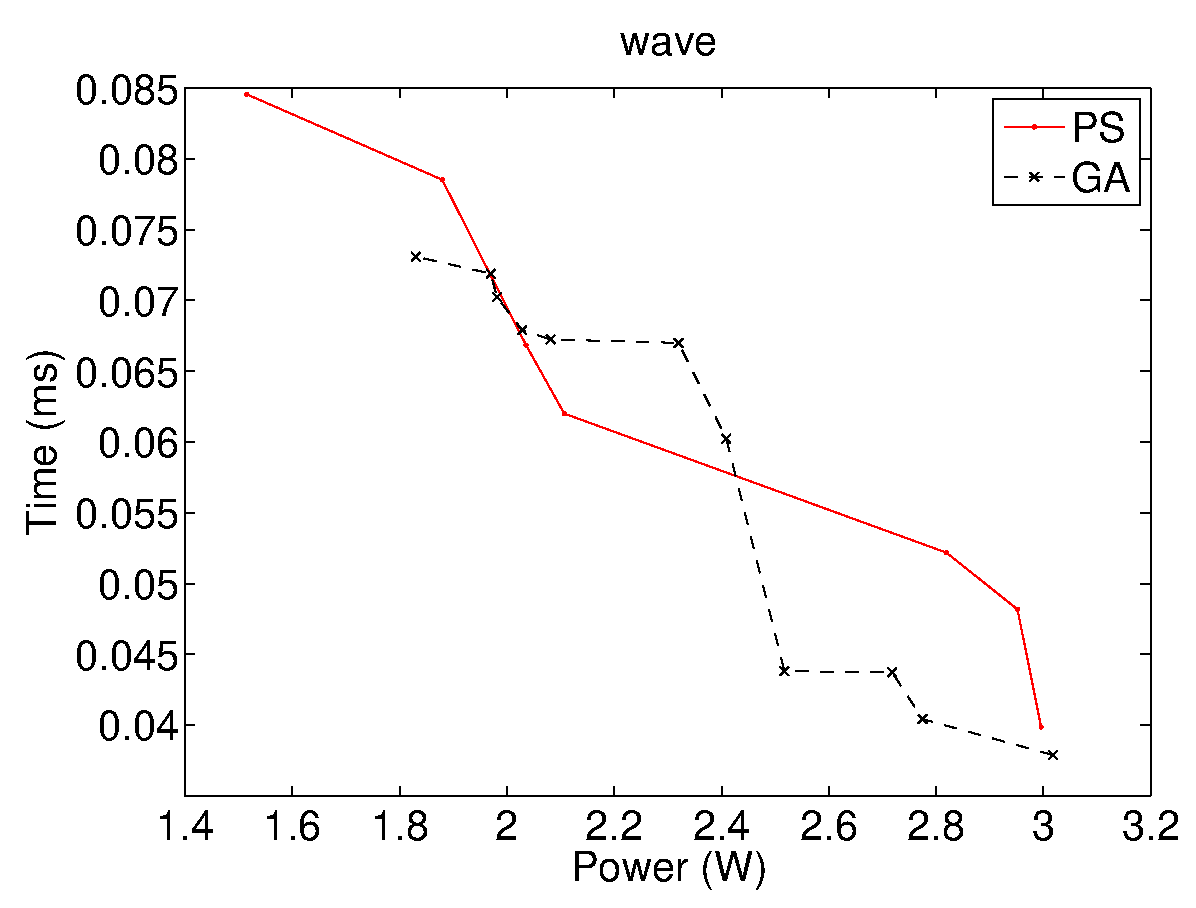
\includegraphics[width=0.30\textwidth]{pictures/wave_100.eps} 
  \end{tabular}
  \caption{Pareto fronts found by PS and GA for a fixed budget of 100 configurations.}
  \label{fig:pareto_fronts_100}
\end{table*}

\begin{table*}
  \centering
  \begin{tabular}{ccc}
    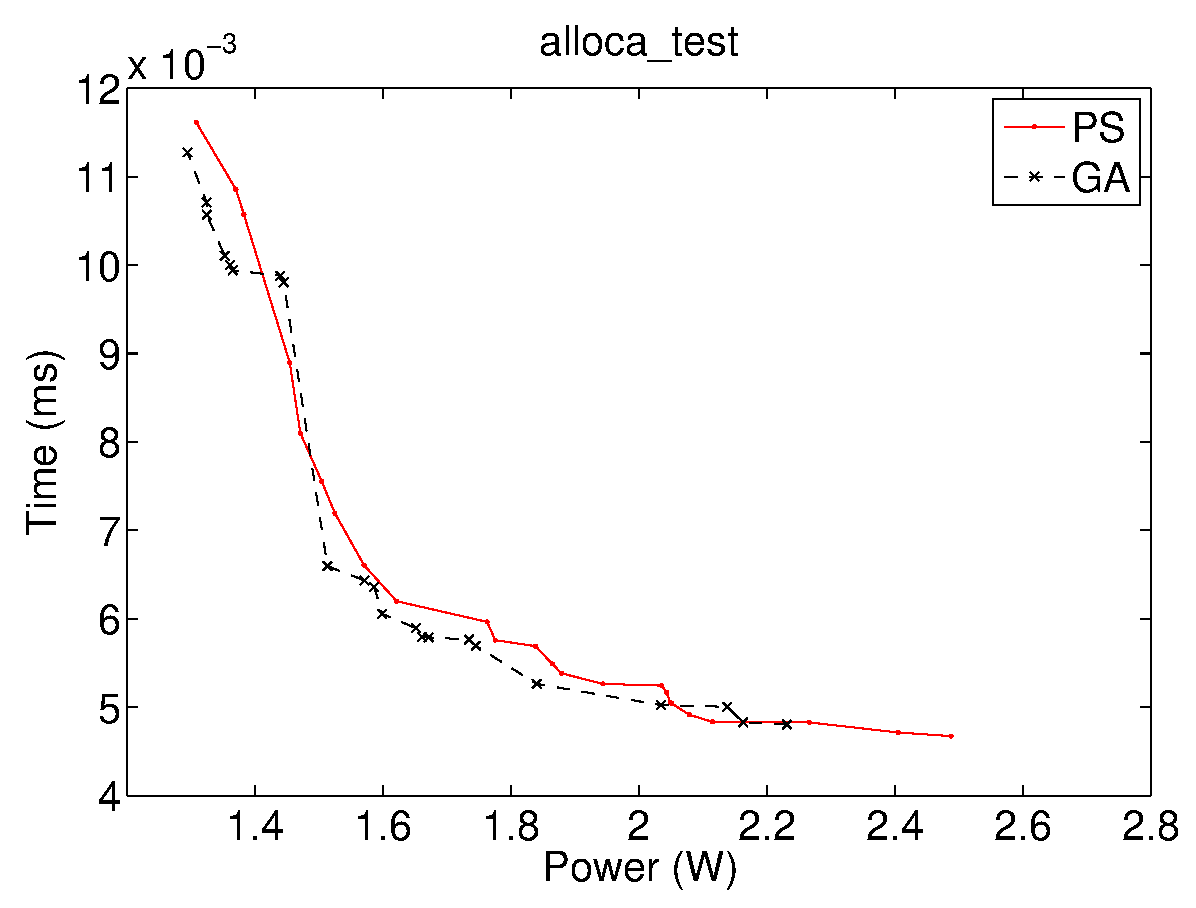
\includegraphics[width=0.30\textwidth]{pictures/alloca_500.eps} &
    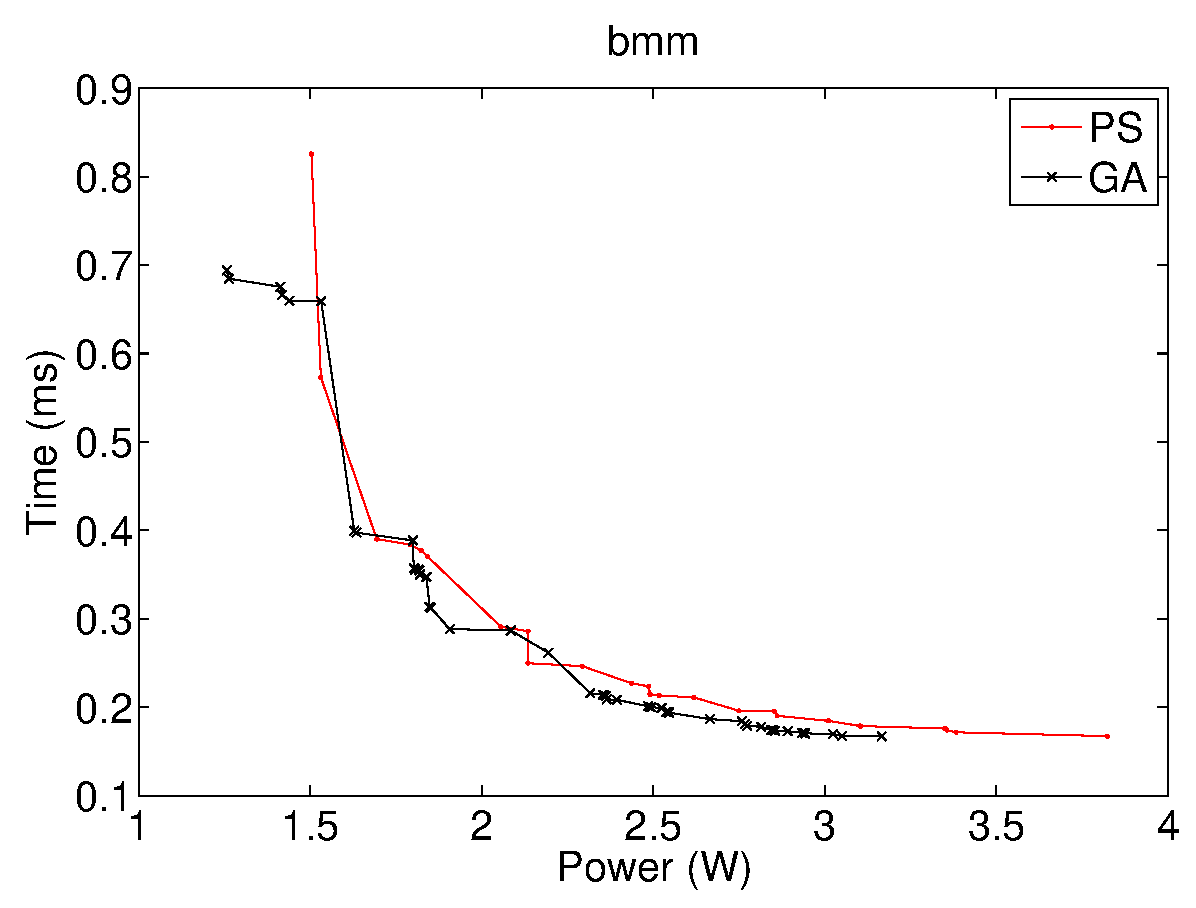
\includegraphics[width=0.30\textwidth]{pictures/bmm_500.eps} & 
    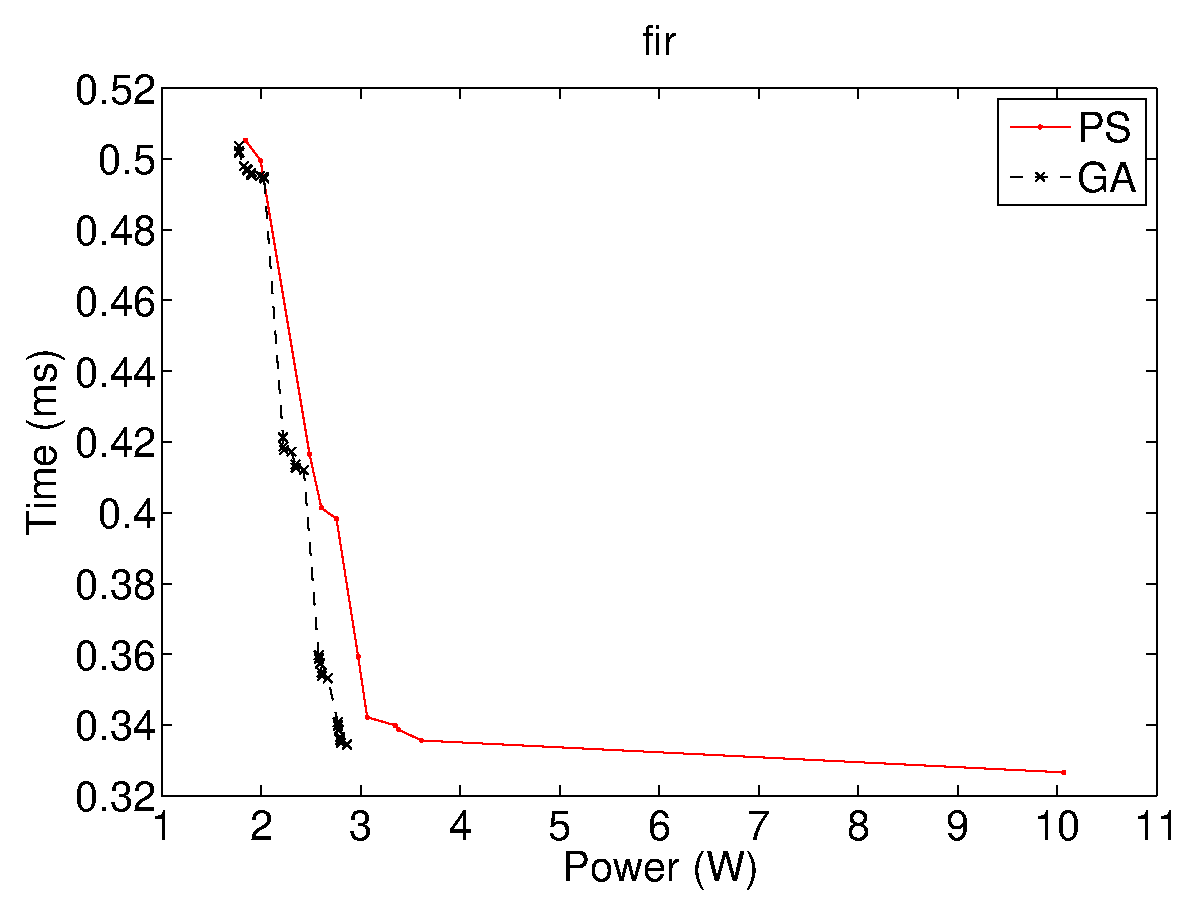
\includegraphics[width=0.30\textwidth]{pictures/fir_int500.eps} \\
    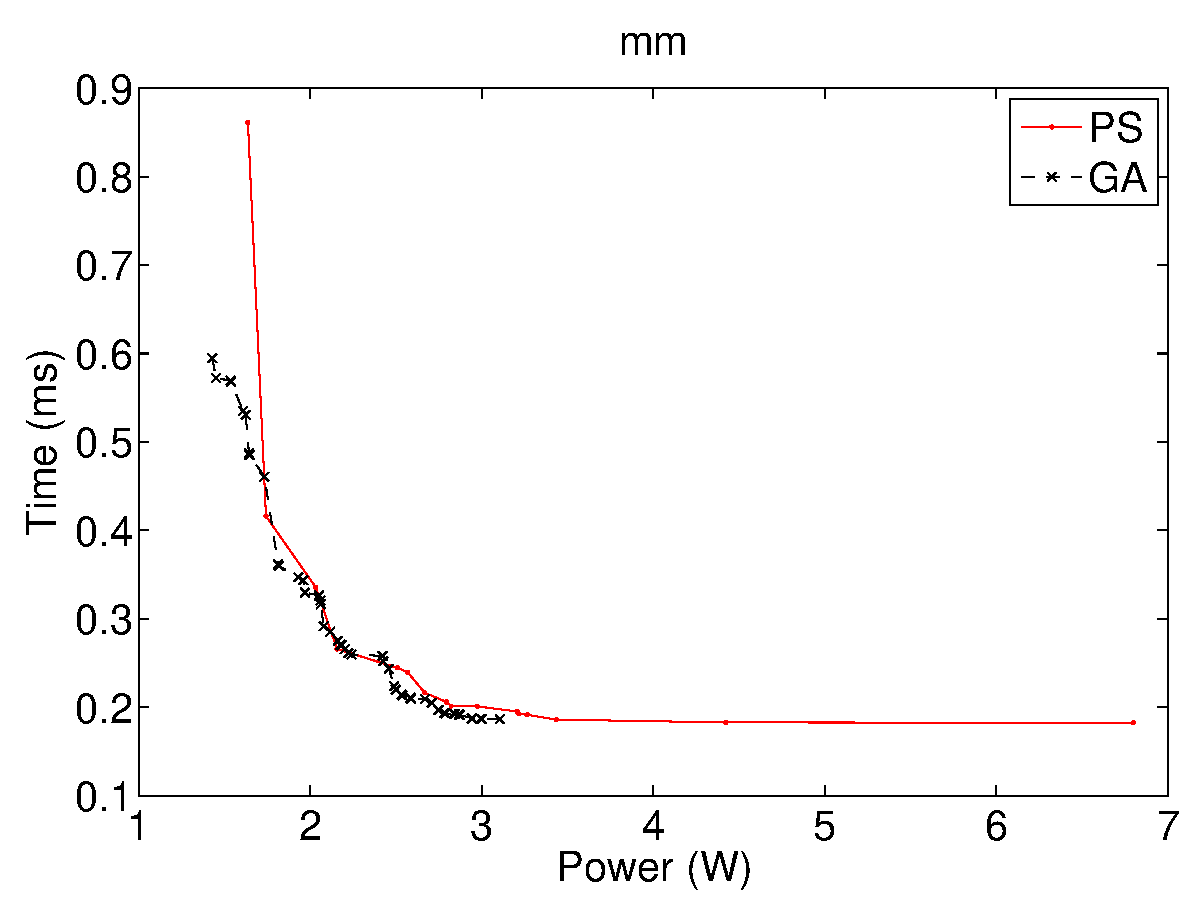
\includegraphics[width=0.30\textwidth]{pictures/mm_500.eps} &
    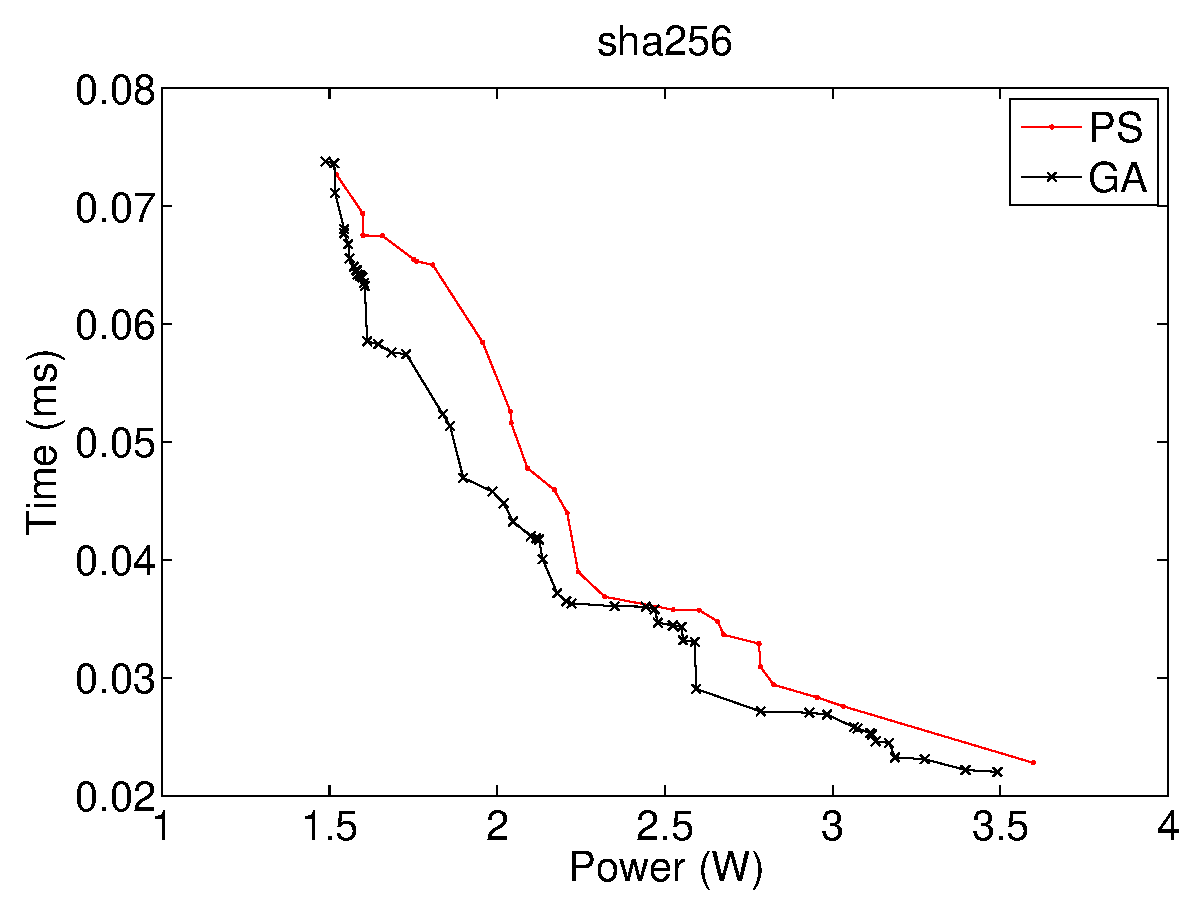
\includegraphics[width=0.30\textwidth]{pictures/sha_500.eps} &
    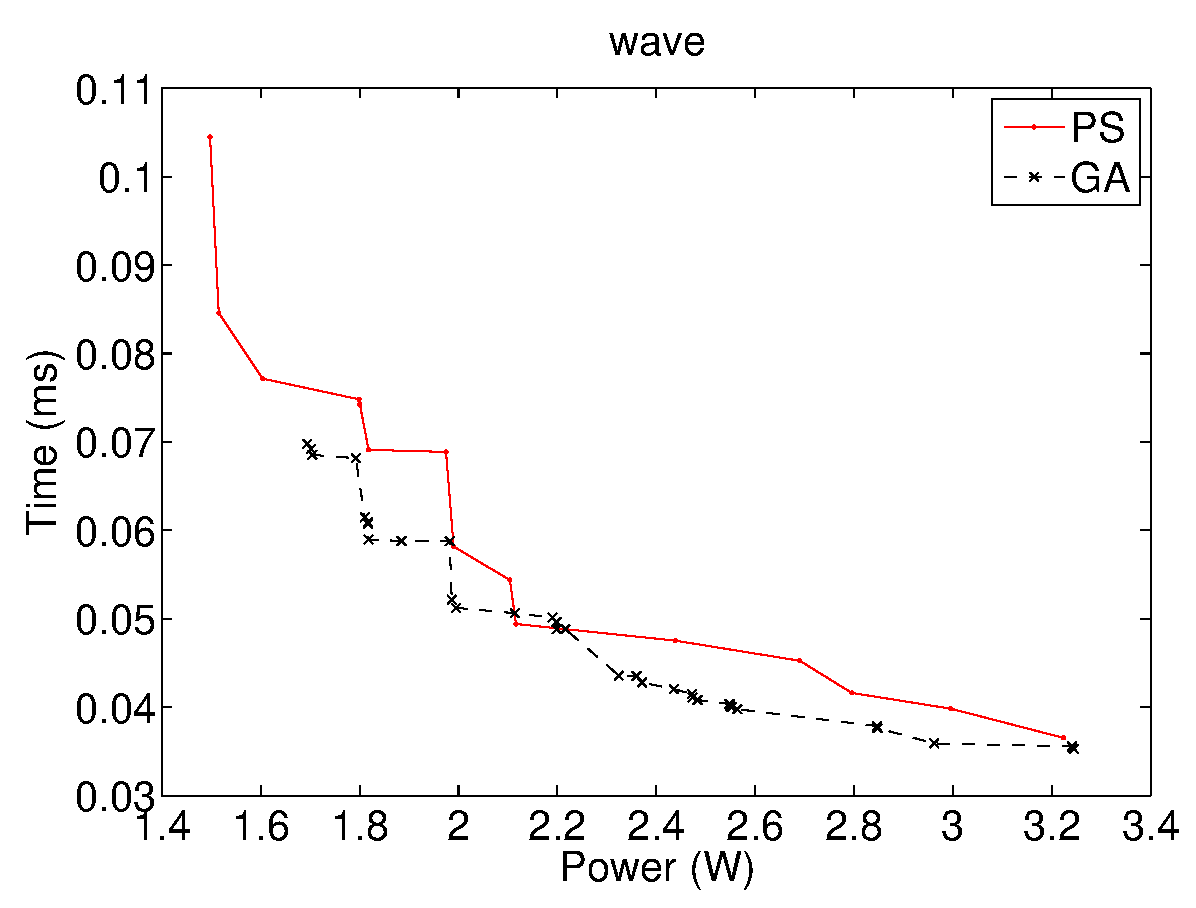
\includegraphics[width=0.30\textwidth]{pictures/wave_500.eps} 
  \end{tabular}
  \caption{Pareto fronts found by PS and GA for a fixed budget of 500 configurations.}
  \label{fig:pareto_fronts_500}
\end{table*}

As can be seen TODO...


In order to evaluate the Paretos from a quantitative point-of-view we
will consider two metrics, namely, the \emph{variation range} and the
\emph{average normalised absolute dispersion error}. For a given
objective, the variation range represents the ratio between the
maximum and the minimum value observed for that objective. A
comparison between the variation range for different benchmarks
between a FCP and a VCP exploration for both power dissipation and
execution time is shown in Fig.~\ref{fig:variation_range}. As it can
be observed, the VCP exploration provides solutions which fall on a
range that is, on average, 23\% and 40\% wider than that provided by a
FCP exploration for power dissipation and execution time,
respectively.
\begin{table}
  \centering
  \begin{tabular}{c}
    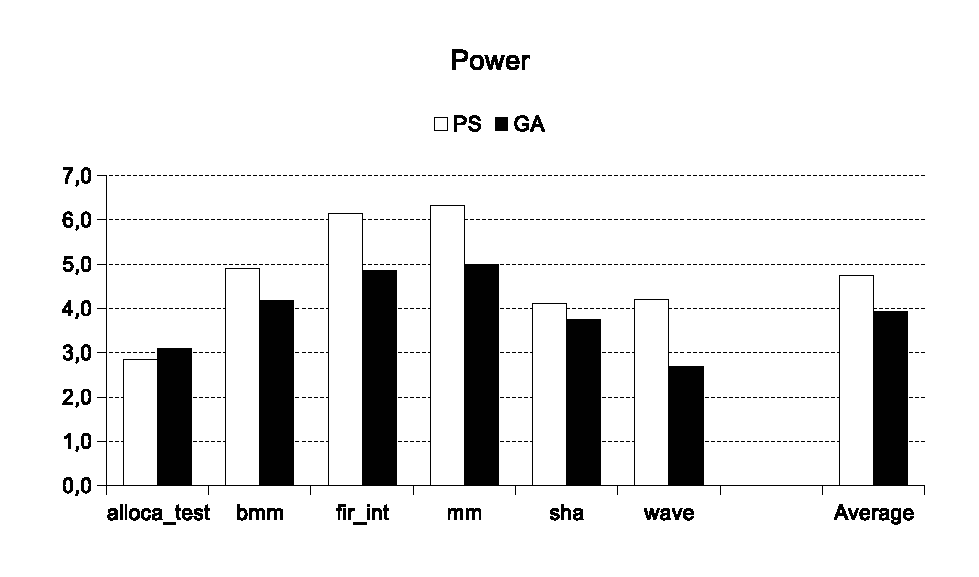
\includegraphics[width=0.4\textwidth]{pictures/variation_power.eps} \\
    (a) \\
    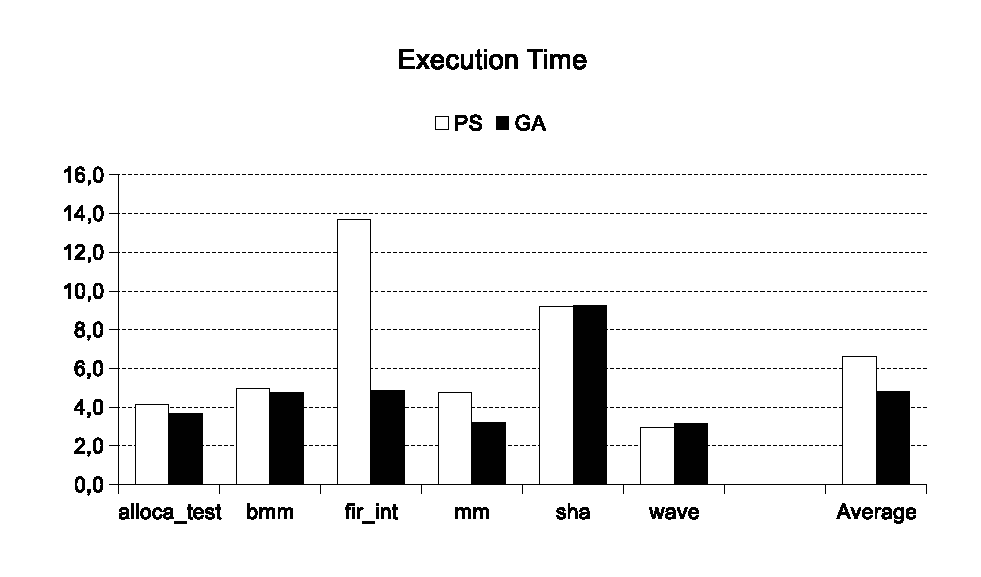
\includegraphics[width=0.4\textwidth]{pictures/variation_etime.eps}
    (b) \\
    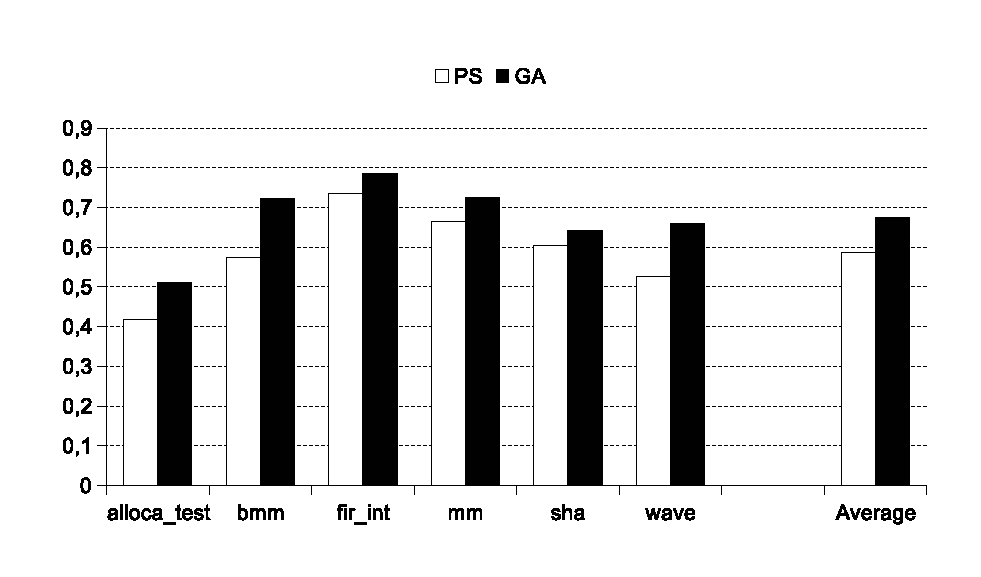
\includegraphics[width=0.4\textwidth]{pictures/dispersion.eps} \\
    (c) 
  \end{tabular}
  \caption{(a)(b) Variation range for different benchmarks between PS and GA
  and average dispersion absolute dispersion (c)}
  \label{fig:dispersion}
\end{table}


The average normalised absolute dispersion error measures
the average absolute difference between the distribution of points in
the objective space and an ideal distribution in which the points are
uniformly distributed over the objective space. Formally, let $O$ be
the image, in the objective space, of the configurations visited by
the design space exploration. The generic element of $O$ (\ie, a
solution) is a pair $(p,t)$ where $p$ and $t$ are the average power
and execution time, respectively. The two-dimensional objective space
is then partitioned by a $M_x \times M_y$ mesh. For each tile $T_i,
\ i=1, 2, \ldots, M_xM_y$ of the mesh, let $N_i$ be the number
of points in $O$ which fall in $T_i$. The average absolute error, $E_i$, for
$T_i$ is the absolute value of the difference between $N_i$ and the
ideal number of solutions, $\overline{N}$, which should fall in $T_i$
in case of uniform distribution. Such $\overline{N}$ can be simply
computed as the ratio between the cardinality of $O$ and the number of
tiles. Thus,
\[ E_i = |N_i - \overline{N}|, \]
where $\overline{N} = |O| / (M_x M_y)$. The average
normalised absolute dispersion error ($ANADE$) is the average of $E_i$
normalised to the maximum absolute error $E_{max}$:
\[ ANADE = \frac{\sum_{i=1}^{M_xM_y} E_i/(M_xM_y)}{E_{max}}, \]
where $E_{max}$ can be computed as the average absolute error in the worst
case in which all the solutions fall in a single tile:
\[ E_{max} = \frac{(M_x M_y - 1) \overline{N} + |\overline{N} -
    |O|| }{M_x M_y}. \] 

Fig.~\ref{fig:dispersion}(c) shows the average normalised absolute
dispersion errors for different benchmarks for FCP and VCP
exploration. As it can be observed, VCP exploration reduces the
dispersion error on average by 20\% as compared to a FCP exporation.

%------------------------------------------------------------------------------

\section{Conclusions}
In this work we presented a multiobjective strategy which 
introduces the concept of Parameter Space representation of Pareto
Set. A case study of a VLIW architecture involving strong
hardware/software dependencies has been carried out to evaluate
effectiveness with different amount of simulations budget.
A qualitative/quantitative comparison against a widespread multiobjective genetic
approach showed how the proposed strategy can result in a different
distribution of Pareto points which trades solutions granularity with
improved pareto extension. 

\balance

\bibliographystyle{IEEEtran} 
\bibliography{bibliography}

% TODO: G2012 bib not used ?

\end{document}
